% ------ headers globales -------------
\documentclass[12pt, a4paper, twoside]{article}
\usepackage{header_tp3}
\raggedbottom % para evitar que se formatee automaticamente "vertically justified" 

%uso: \ponerGrafico{file}{caption}{scale}{label}
\newcommand{\ponerGrafico}[4]
{\begin{figure}[H]
	\centering
	\subfloat{\includegraphics[scale=#3]{#1}}
	\caption{#2} \label{fig:#4}
\end{figure}
}

%\includeonly{instrucciones, codigo-fuente, conclusiones, introduccion, problema1, problema2, problema3}
\begin{document}{}
% -------------------------------------
% -- Carátula --
\newpage{\pagestyle{empty}% parametros para la caratula (caratula.sty)

\materia{Algoritmos y Estructuras de Datos III}
\submateria{Entrega de TP}
\titulo{Trabajo Práctico 2}
\subtitulo{Técnicas Algorítmicas Avanzadas}
\fecha{Viernes 9 de Mayo de 2014}
\integrante{Barrios, Leandro E.}{404/11}{ezequiel.barrios@gmail.com}
\integrante{Benegas, Gonzalo}{958/12}{gsbenegas@gmail.com}
\integrante{Duarte, Miguel}{904/11}{miguelfeliped@gmail.com}
\integrante{Niikado, Marina}{711/07}{mariniik@yahoo.com.ar}
\grupo{Grupo \red{\texttt{$(-1111111111111111111111111111111111111111111111111111111111111001_{2})$}}}

\maketitle\cleardoublepage}
  % -- nota:
  %       si no esta dentro de \newpage{} se rompe la numeracion y el encabezadp
  %       \cleardoublepage es para que el indice no se imprima atras de la caratula
%~ \pagestyle{empty}% parametros para la caratula (caratula.sty)

\materia{Algoritmos y Estructuras de Datos III}
\submateria{Entrega de TP}
\titulo{Trabajo Práctico 2}
\subtitulo{Técnicas Algorítmicas Avanzadas}
\fecha{Viernes 9 de Mayo de 2014}
\integrante{Barrios, Leandro E.}{404/11}{ezequiel.barrios@gmail.com}
\integrante{Benegas, Gonzalo}{958/12}{gsbenegas@gmail.com}
\integrante{Duarte, Miguel}{904/11}{miguelfeliped@gmail.com}
\integrante{Niikado, Marina}{711/07}{mariniik@yahoo.com.ar}
\grupo{Grupo \red{\texttt{$(-1111111111111111111111111111111111111111111111111111111111111001_{2})$}}}

\maketitle 
\setcounter{page}{1}

%-- Índice --
\newpage{\pagestyle{empty}\tableofcontents\cleardoublepage}

%-- Dentro de TP3 redefino ciertos comandos para que se pueda compilar todo individualmente --
\begin{TP3}
%-- Introduccion --
\section{Introducción}\label{sec:introduccion}

En este trabajo pr\'actico nos piden analizar el problema del \textit{Camino Acotado de Costo M\'inimo} ($CACM$), y desarrollar distintos algoritmos para resolverlo. 

Dado un Grafo $G = (V,E)$, dos funciones de peso $\omega_1, \omega_2: V \mapsto \mathbb{R}_+$, un natural $K$ y dos nodos $u,v \in V$, el problema consiste en encontrar, entre todos los caminos $P$ entre $u$ y $v$ que cumplen $\omega_1(P) \leq K$, el que minimice $\omega_2(P)$. 

Donde si $w$ es una función de peso definida sobre aristas, se entiende $w(P)$ como 

\begin{equation*}
\sum_{e \text{ arista de } P} w(e)
\end{equation*}

$CACM$ es un problema conocido, y tiene muchas aplicaciones en la vida real. Una agencia de vuelos puede estar interesada en ofrecer el viaje más corto entre dos ciudades, dado un cliente con un presupuesto acotado. Los nodos representan ciudades. $u$ y $v$ son las ciudades de origen y destino, respectivamente. Una arista es un vuelo particular entre dos ciudades. El peso por $\omega_1$ es el costo del pasaje y el peso por $\omega_2$  es la duración del vuelo. Un camino es una secuencia de vuelos, es decir, un vuelo que puede o no tener escalas. K viene a ser el presupuesto del cliente. El camino buscado es entonces el que, entre todos los vuelos (con o sin escalas) entre la ciudad de origen y destino que el cliente puede pagar, tiene la menor duración.

Otro ejemplo similar está relacionado con el Mapa Interactivo de la Ciudad de Buenos Aires. Se busca llegar de un punto de la ciudad a otro en el
menor tiempo, aunque se puede especificar la máxima cantidad de metros por caminar. Los nodos son alturas de calles, es decir puntos geográficos sobre alguna calle. Una arista entre dos nodos es un segmento de calle - junto con un medio de transporte - que une dos puntos geográficos. El peso por $\omega_1$ es la longitud del segmento si el medio de transporte es `caminar' y 0 si no. El peso por $\omega_2$ es el tiempo que demora recorrer el segmento usando el correspondiente medio de transporte. El valor K, especificado por el usuario, es la máxima cantidad de metros que está dispuesto a caminar. Un camino entre un punto $u$ de origen a otro punto $v$ de destino es una sucesión de segmentos recorridos con un correspondiente medio de transporte. Se busca, entre todos los caminos cuyos metros caminados totales no exceden K, el de menor duración.

Un ejemplo reciente fue obtenido del \textit{MIT Technology Review}\footnote{technologyreview.com/view/528836/forget-the-shortest-route-across-a-city-new-algorithm-finds-the-most-beautiful/}. \fixme{guarda que este es maximo, explicar}

Aunque $CACM$ es un problema conocido, no se conocen algoritmos polinomiales que lo resuelvan y se estima que pertenece al conjunto de problemas NP. En este trabajo se analizaran varios métodos para resolverlo: una soluci\'on exacta y 5 aproximaciones a trav\'es de heur\'isticas. En concreto, se implementarán los siguientes algoritmos:

\begin{enumerate}
\item Un \textit{Backtracking} como algoritmo exacto.
\item Una heur\'istica \textit{constructiva greedy}.
\item Una heur\'istica de \textit{b\'usqueda local}.
\item Una heur\'istica \textit{GRASP}.
\end{enumerate}

El enfoque estará puesto en experimentar sobre cada uno de estos algoritmos, analizando su complejidad y la calidad de las solucion en el caso de las heur\'isticas.
Se intentará definir diferentes familias de grafos sobre los cuales poder obtener resultados concluyentes sobre el comportamiento del algoritmo.

\newpage
%-- Instrucciones --
\section{Instrucciones de uso}\label{sec:instrucciones}
Para compilar el proyecto completo: entrar en la carpeta \texttt{src} y correr \texttt{make all}.

Para compilar cada una de las partes por separado: en la carpeta \texttt{src}, estan las carpetas \texttt{backtracking}, \texttt{grasp}, \texttt{greedy\_heuristic\_\{A,B,C\}} y \texttt{local\_search}. Se puede compilar cada parte de forma independiente, entrando en cada carpeta y ejecutando \texttt{make}. 

Funcionamiento de los archivos \texttt{Makefile}:

\begin{itemize}
    \item Hay un archivo \texttt{Makefile.common} que se usa como input para los \texttt{Makefile} del resto de las carpetas.
  La sintaxis para incluirlo es: \texttt{include ../Makefile.common}
  
  \item Por defecto, compila el archivo que tenga el mismo nombre de la carpeta, y busca el \texttt{.cpp} y el \texttt{.h}.
      Por ejemplo, si estamos en la carpeta \texttt{backtracking} va a buscar \texttt{backtracking.cpp} y \texttt{backtracking.h} y lo va a compilar en \texttt{backtracking}.
	  
  \item Siempre va a crear una carpeta \texttt{OBJS} en donde guarda los archivos \texttt{.o}
  
  \item Cuando se desean incluir archivos que se encuentren en la carpeta \texttt{common}, se debe anteponer \texttt{COMMON\_OBJS} al \texttt{include}:
  
  \begin{verbatim}
      COMMON\_OBJS := ClassName1 ClassName2
      include ../Makefile.common
  \end{verbatim}
  
  en donde \texttt{ClassName} es el nombre de la clase. Por ejemplo, \texttt{COMMON\_OBJS := Graph Edge}

  \item Se pueden agregar targets específicos que luego del \texttt{include ../Makefile.common}.
  
\end{itemize}

\newpage

%-- Desarrollo --
\section{Desarrollo del TP}\label{sec:desarrollo}
  
  %-- Backtracking --
  \subsection{Backtracking}\label{subsec:backtracking}
  \subsubsection{Descripción}

El algoritmo a cada paso tiene un camino $P = [v_1 = u, \dots, v_{i-1}]$ e intenta agregar al camino un nuevo nodo $v_i$ de la adyacencia de $v_{i-1}$, hasta que llega al nodo destino $V$. De esta forma recorre todos los caminos entre $U$ y $V$. De entre todos los caminos tales que el peso por $\omega_1$ es menor o igual a K, se guarda el de menor $\omega_2$.

Se implementaron las siguientes podas:

\begin{itemize}
    \item Se exploran solamente caminos simples. Si un camino tiene ciclos, removiéndolo se obtiene uno con menor longitud tanto en $\omega_1$ como en $\omega_2$. Por lo tanto la solución que buscamos no puede tener ciclos, y nos restringimos a caminos simples. La poda se implementó guardando un arreglo que marca para cada nodo si es parte del camino o no. No se agrega nuevamente si ya es parte del camino.
    \item Si el camino parcial $P = [v_1 = u, \dots, v_{i-1}]$ cumple:

        $omega_1(P)$, sumado a la distancia según $\omega_1$ entre $v_{i-1}$ y $V$, es mayor que $K$

entonces se abandona la rama, es decir, no se recorren los caminos que empiezan en $P$, ya que cualquiera de éstos no va a cumplir con la restricción de que $omega_1$ sea menor o igual a $K$.
    \item Si el camino parcial $P = [v_1 = u, \dots, v_{i-1}]$ cumple:

        $omega_2(P)$, sumado a la distancia según $\omega_2$ entre $v_{i-1}$ y $V$, es mayor o igual que el peso según $\omega_2$ del mejor camino encontrado hasta el momento

entonces se abandona la rama, es decir, no se recorren los caminos que empiezan en $P$, ya que cualquiera de éstos no va a proporcionar una solución mejor que la ya encontrada.
\end{itemize}

A continuaci\'on, el pseudoc\'odigo de la funci\'on \texttt{backtrack}.

\begin{algorithm}[H]
    \caption{\texttt{backtrack}(Edge e)}
\begin{algorithmic}[1]
  \State Node n $\leftarrow$ e.toNode
  \State currentBranch.path.push\_back(n)
  \State currentBranch.totalOmega1 += e.omega1
  \State currentBranch.totalOmega2 += e.omega2
  \State visited[n] $\leftarrow$ true
  \State podar $\leftarrow$ currentBranch.totalOmega1 + distanceToVOmega1[n] $>$ K \textbf{or} currentBranch.totalOmega2 + distanceToVOmega2[n] $\geq$ bestSolutionFound.totalOmega2
  \If{\textbf{not} podar}
  \If{n = V}
      \State bestSolutionFound $\leftarrow$ currentBranch
  \Else{}
      \For{\textbf{each} Node a \textbf{in} adjacencyList[n] }
	\If{\textbf{not} visited[a] }
          \State Edge f = incidencyMatrix[n][a]
          \State backtrack(f)
	\EndIf
      \EndFor
  \EndIf
  \EndIf
  \State currentBranch.path.pop\_back()
  \State currentBranch.totalOmega1 -= e.omega1
  \State currentBranch.totalOmega2 -= e.omega2
  \State visited[n] $\leftarrow$ false
\end{algorithmic}
\end{algorithm}

\subsubsection{Complejidad}

\fixme{hacer, te tiene que dar (n+1)!}
%Analicemos cuantas llamadas se hacen a $backtrack$. Se exploran caminos de a los sumo $n$ nodos. El primer nodo está fijo en $u$. El segundo nodo
%pertenece a la adyacencia del primero, que en peor caso tiene tamaño $n - 1$. El tercero pertenece a la adyacencia del segundo, que no hayan sido
%visitados, cuyo tamaño es a lo sumo $n - 2$. Y asi sucesivamente. En peor caso se llama a $backtrack$ $n!$ veces.
%
%Analicemos el cómputo que se realiza en cada llamada a $backtrack$. Preguntar si un nodo está visitado es acceder a un arreglo en forma constante.
%El costo de una función de peso asociada a un camino se va acumulando a medida que se agregan nodos. El costo se guarda y se puede acceder en
%forma constante. Lo queda por estudiar es la complejidad del ciclo $for$ que recorre la adyacencia del nodo visitado. Guardamos una lista de
%adyacencia por lo que podemos recorrer la adyacencia de cualquier nodo con complejidad lineal en relación a su tamaño. El tamaño de la adyacencia
%es a lo sumo $m$. Para cada nodo adyacente se efectúan operaciones constantes, a excepción de las llamadas a $backtrack$. El costo de estas
%llamadas lo estamos calculando por separado.
%
%En definitiva hacemos $O(n!)$ llamadas a una función que de por si toma $O(m)$ operaciones. La complejidad del algoritmo es $O(m*n!)$.

\subsubsection{Experimentación}

\fixme{hacer}
%Generamos en primera instancia grafos con una cantidad de nodos pequeña - entre 3 y 15. La cantidad de aristas, es decir, la densidad del grafo,
%se eligió aleatoriamente entre 0 y (n * (n - 1)) / 2, la cantidad máxima posible. La distribución de las aristas, sus pesos, y el valor de $k$
%también se eligieron de forma aleatoria.
%
%A continuación presentamos los tiempos de ejecución de nuestro algoritmo frente a estas instancias. 
%
%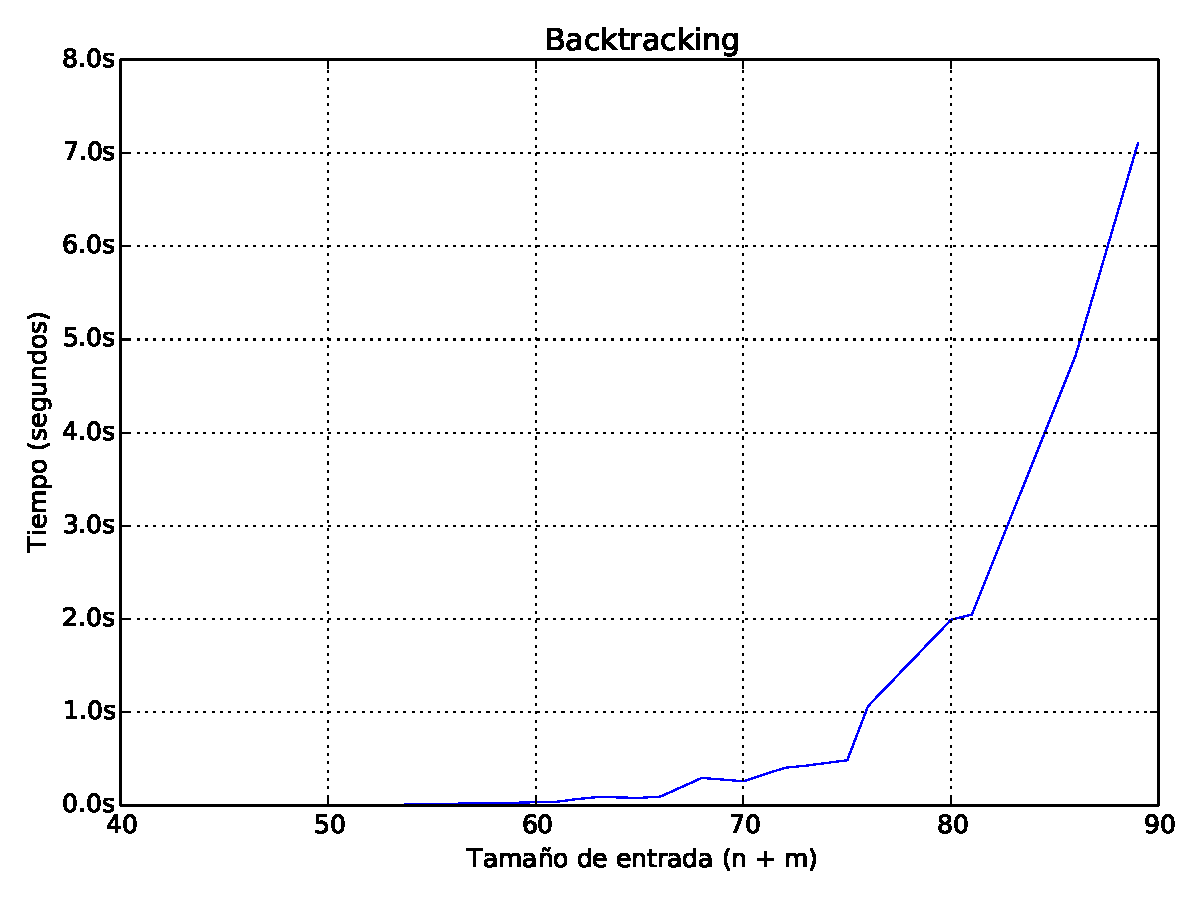
\includepdf[pages={1}]{imagenes/backtracking-aleatorio.pdf}
%
%Para tamaños de grafo menores que 40, los tiempos de ejecución fueron despreciables. Se puede apreciar el carácter exponencial del tiempo de
%ejecución de nuestro algoritmo en función del tamaño de entrada.

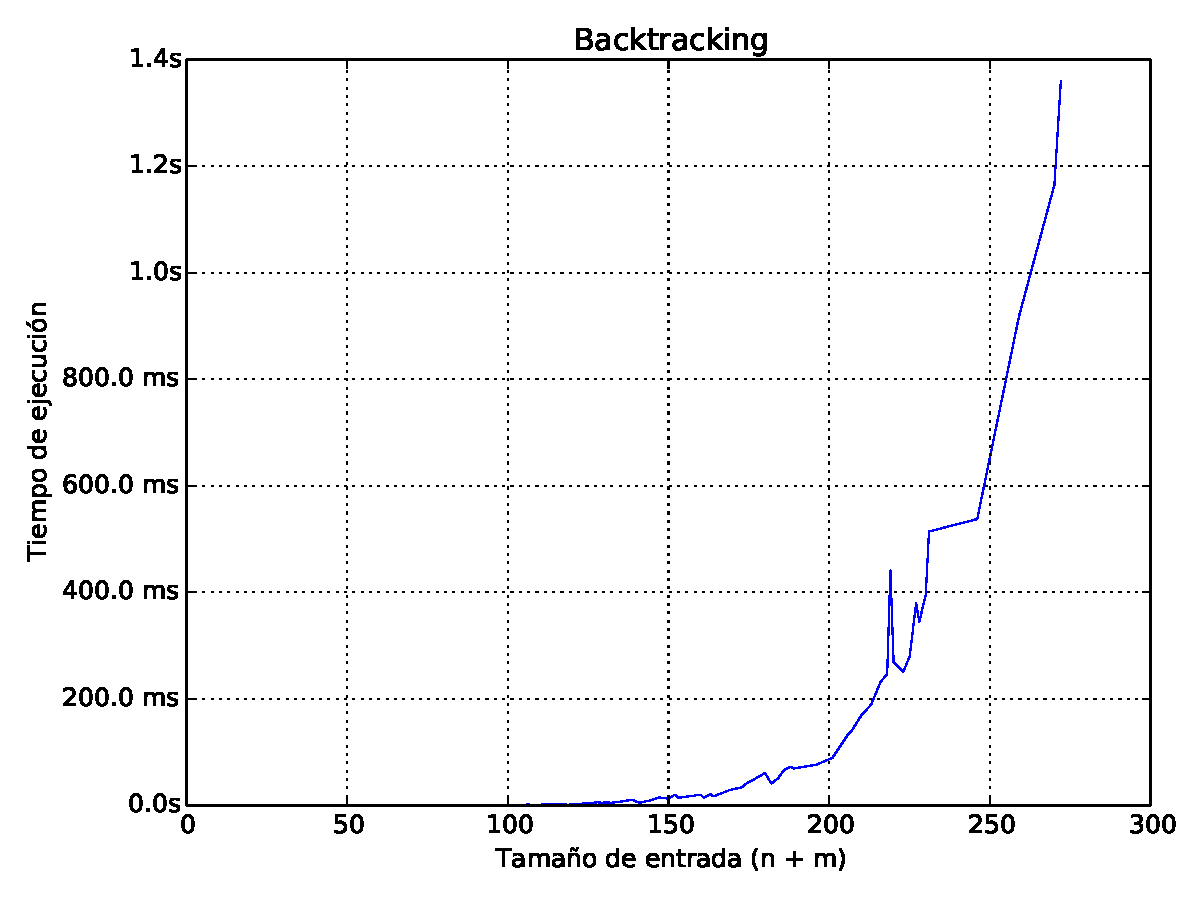
\includepdf[pages={1}]{imagenes/backtracking-complejidad-general.pdf}

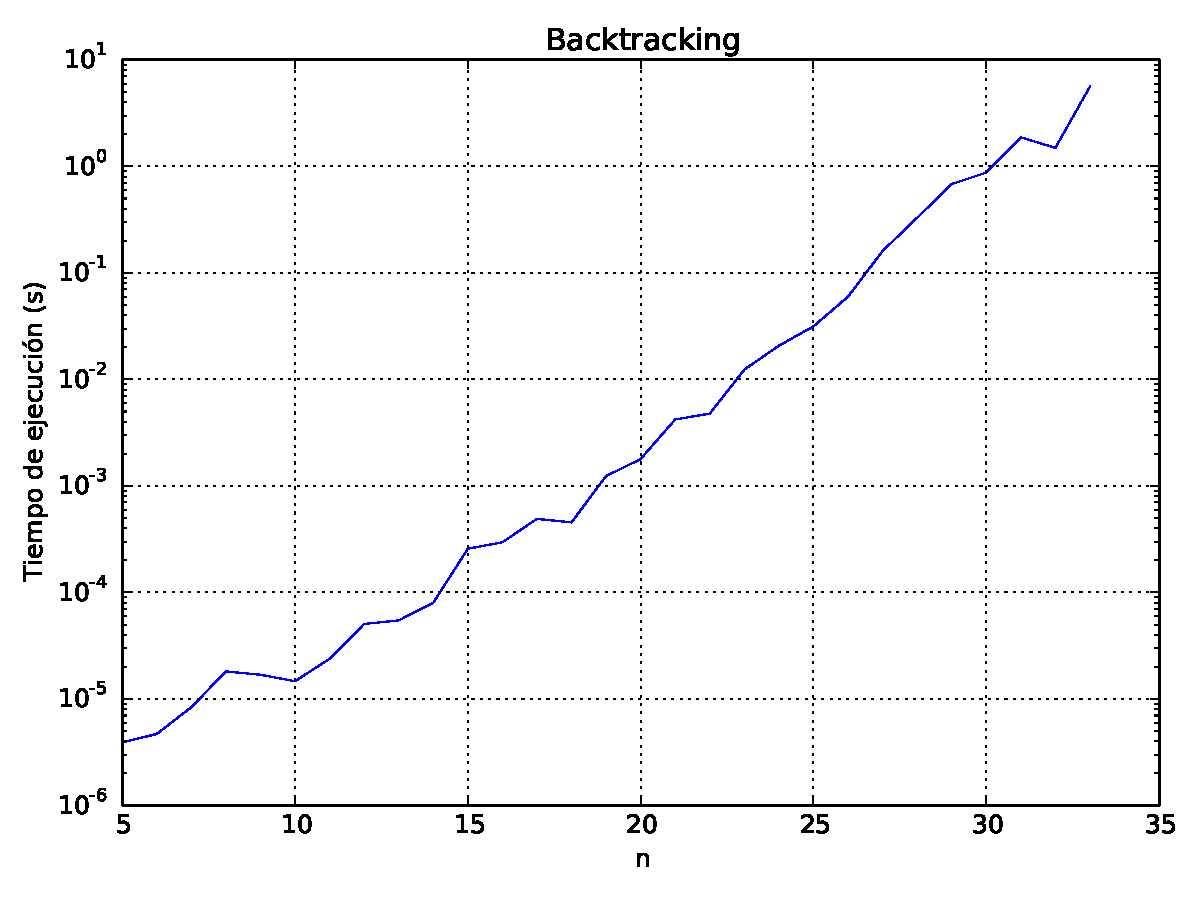
\includepdf[pages={1}]{imagenes/backtracking-complejidad-funcion-de-n.pdf}

aca m valio siempre la mitad del maximo, o sea n(n-1)/4

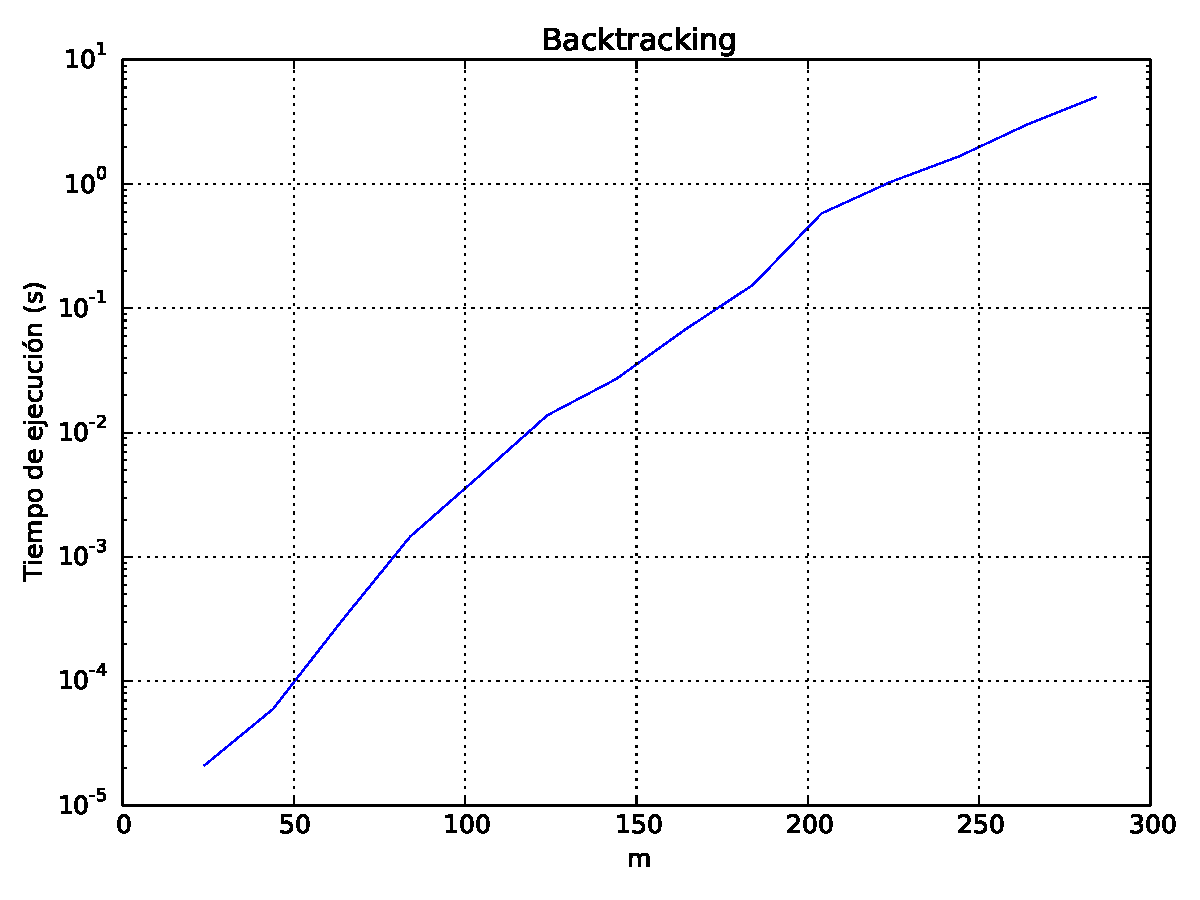
\includepdf[pages={1}]{imagenes/backtracking-complejidad-funcion-de-m.pdf}

se tomo n = 25, y se varió desde el mínimo de este grafo (n-1) hasta el completo

  \newpage

  %-- Greedy --
  \subsection{Greedy}\label{subsec:greedy}
  
Para resolver un problema, un algoritmo goloso sigue una heur\'istica que consiste elegir en cada paso, entre un conjunto de opciones, una soluci\'on \'optima local, esperando encontrar al final la soluci\'on \'optima global. En general estos algoritmos son eficientes y simples de dise\~nar e implementar, pero puede ser que nunca lleguen a la soluci\'on \'optima del problema. 

De acuerdo a la definici\'on de Brassard\footnote{\label{Brassard}Brassard G., Bratley P., {\it Fundamental of Algorithmics}, Prentice Hall, 1996. (c)}, un algoritmo goloso se compone de los siguientes elementos: 

\begin{enumerate}
 \item Un conjunto de candidatos que ya han sido considerados y seleccionados. 
 \item Un conjunto de candidatos considerado y rechazados. 
 \item Una funci\'on que comprueba si cierto conjunto de candidatos constituye una soluci\'on a nuestro problema, ignorando si es o no \'optima por el momento. 
 \item Una funci\'on de factibilidad, que me dice si es posible o no completar el conjunto a\~nadiendo otros candidatos para obtener al menos una soluci\'on de nuestro problema. 
 \item Una funci\'on selecci\'on que indica en cualquier momento cu\'al es el m\'as prometedor de los candidatos restantes, que no han sido seleccionados ni rechazados. 
 \item Una funci\'on objetivo, que da el valor de la soluci\'on que hemos hallado. 
\end{enumerate}

Lo que busca el algoritmo goloso es encontrar el conjunto de candidatos que constituya una soluci\'on, y que optimice el valor de la funci\'on objetivo. Este algoritmo avanza paso a paso. Inicialmente, el conjunto de elementos seleccionados est\'a vac\'io. Entonces, en cada paso se considera a\~nadir a este conjunto el mejor candidato sin coniderar los restantes, de acuerdo a nuestra funci\'on selecci\'on. Si el conjunto ampliado de candidato seleccionados ya no fuera factible, rechazamo el candidato que estamos considerando en ese momento. Sin embargo, si el conjunto aumentado sigue siendo factible, entonces a\~nadimos el candidato actual al conjunto de candidatos selecccionados, en donde pasar\'a a estar desde ahora en adelante. Cada vez que se ampl\'ia el conjunto de candidatos seleccionados, comprobamos si \'este constituye ahora una soluci\'on para nuestro problema. A partir de este esquema, al agregar siempre subsoluciones \'optimas a mi conjunto, al finalizar lo que se espera encontrar es la soluci\'
on \'optima. 

El algoritmo de Dijsktra para encontrar caminos m\'inimos en un grafo pesado es un algoritmo goloso, que funciona y es correcto, como lo fue demostrado por Bassard en el libro mencionado.

Dado un grafo $G=(V,X)$, Dijkstra guarda un conjunto $S$ de nodos que ya fueron recorridos y un vector $\pi$ con la distancia m\'inima de un nodo $u$ a todos los de $S$. En cada fase de Dijkstra, se selecciona un nuevo nodo de $V\backslash S$ cuyo valor en $\pi$ sea m\'inima y lo a\~nadimo a $S$, actualizando si es necesario $\pi$. Al finalizar, $\pi$ es el vector con la m\'inima distancia a todos los nodos. 

Entonces, nosotros para resolver el problema vamos implementar Dijkstra con tres funciones objetivo diferentes, que toman una arista y devuelven un peso para ella: 

\begin{enumerate}
  \item $f_A(e) = \omega_1(e)$
  \item $f_B(e) = \omega_2(e)$
  \item $f_C(e) = \omega_1(e)\omega_2(e)$
\end{enumerate}

Luego el pseudoc\'odigo de Dijkstra modificado con la nueva definici\'on de distancia queda dado por: 

\begin{algorithm}
In: Grafo $G = (V,X)$, nodo inicial $v_0$, ObjectiveFunction $f$ \newline
Out: Arreglo $\pi$ con camino m\'inimo en funci\'on de $f$ a cada nodo. 
\begin{algorithmic}[1]
\State $\pi(v) = \infty$ \quad $\forall v \in V$
\State $\pi(v_0) = 0$
\State $S = \emptyset$
\For{$i = 1 \dots n-1$}
    \State $v \leftarrow $ nodo de $V\backslash S$ de m\'inimo $\pi$. 
    \For{{\bf each} $w \in V\backslash S$ adyacente a $v$}
      \State $\pi(w) = \min( \pi(w), \pi(v) + f((v,w)))$
    \EndFor
    \State $S = S \cup \{v\}$
\EndFor
\State \textbf{retornar} $\pi$
\end{algorithmic}
\end{algorithm}

La modificaci\'on est\'a la l\'inea 7, que en vez de sumar a $\pi(v)$ el peso de la arista, como es en el algoritmo original, le suma el valor de una funci\'on que define el peso de la arista. Esto nos permite mucha flexibilidad a la hora de cambiar la ``decisi\'on golosa''.

%-- Goloso A --
\clearpage
\subsubsection{Greedy A}\label{subsubsec:greedy-a}
Dado un grafo $G = (V,E)$, obtenemos el camino m\'inimo entre $u$ y $v$ seg\'un $\omega_1$. 

Familias malas
\ponerGrafico{imagenes/maloGreedyA.png}{}{0.5}{malo-para-greedy-a}

Para ir de 1 a 4 hay dos caminos posibles: ($C_1$) $1 \rightarrow 2 \rightarrow 4$; ($C_2$) $1 \rightarrow 3 \rightarrow 4$

\begin{eqnarray}
 \omega_1(C_1) &=& 2 	\\ 
 \omega_2(C_1) &=& 2x	\\
 \omega_1(C_2) &=& 2x	\\
 \omega_2(C_2) &=& 2
\end{eqnarray}

%-- Goloso B --
\clearpage
\subsubsection{Greedy B}\label{subsubsec:greedy-b}
Dado un grafo $G = (V,E)$, obtenemos el camino m\'inimo entre $u$ y $v$ seg\'un $\omega_2$. 

\clearpage
%-- Goloso C --
\subsubsection{Greedy C}\label{subsubsec:greedy-c}
Dado un grafo $G = (V,E)$, obtenemos el camino m\'inimo entre $u$ y $v$ seg\'un $\omega_1\omega_2$. 

  \newpage

  %-- Local Search --
  \subsection{Local Search}\label{subsec:local}
  % ------ headers globales y begin ---------------
\documentclass[11pt, a4paper, twoside]{article}
\usepackage{header_tp3}
\begin{document}{}
% -----------------------------------------------

% Búsqueda local

% Explicación inicial

% Solución inicial
Partimos desde una solución factible obtenida a partir de un algoritmo goloso. En caso de que el algoritmo anterior no devuelva una solución factible, corremos Dijkstra utilizando la sumatoria de los pesos $\omega_1$ como función objetivo. Si Dijkstra tampoco devuelve una solución factible, podemos asegurar que no existe solución al problema\footnote{Demostrado en la sección de heurística golosa}. En este caso, devolvemos ``no''.

Solución Inicial 2:
Corro dijkstra con omega1 y omega2, formando $c_1$ y $c_2$. Tomo el conjunto $U$ de nodos formados por $c_1 \cap c_2$. Para cada par de nodos $n_1,n_2$ adyacentes, me fijo si puedo formar un camino mejor valuado en $\omega_2$ reemplazando el camino $c^1_{n_1,n_2}$ por $c^2_{n_1,n_2}$, siempre que el nuevo camino no se pase de K al valuarlo en $\omega_2$. La evaluación se hace ordenando por omega2, de forma tal que el camino obtenido sea el que minimice la misma en comparación con el resto de los posibles caminos que se podrían obtener con este método.

\begin{comment}

% Definición de vecindad
Vecindad <<A>>: 

Dado el grafo inicial G, y una solución formada por un camino $c \in G$, definimos sus soluciones vecinas como aquellas resultantes de tomar un subcamino $d_{n_1,n_2} \in c$ entre dos pares de nodos $n_1,n_2$ cualesquiera, y reemplazarlo por un camino ``mejor'' $d_{n_1,n_2}^* \in G$, de tal forma que el camino $c^* = c - d_{n_1,n_2} + d_{n_1,n_2}^*$ resultante cumpla: 
\begin{list}
\item $\omega_1(c^*) \leq k $
\item $\omega_2(c^*) < \omega_2(c)$
\end{list}

Dada una solución $S$ formada por un camino $c$ definimos su vecindad como el conjunto $S^*$ de todos los caminos $c^*$ posibles.

% Selección de vecino
Dada una vecindad $S^*$, se probaron los siguientes métodos de elegir al vecino:
\begin{list}
	\item Steepest descent, con $\omega_2$ como función objetivo.
	\item Steepest descent, con $\omega_1*\omega_2$ como función objetivo.
	\item Elegir el primero que se encuentre.
	\item Stochastic \fixme{completar} eligiendo el vecino de forma pseudoaleatoria.
\end{list}

\end{comment}

% -----------------------------------------------
\end{document}
  \newpage

  \subsection{GRASP}\label{subsec:grasp}
  %Grasp
La metaheurística Grasp consiste en generar varias soluciones iniciales a partir de una heurística golosa aleatorizada y correr búsqueda local sobre ellas. La solución final es la mejor encontrada tras todas las búsquedas locales.
Sea $S$ el conjunto de soluciones iniciales, el algoritmo que se usa es el siguiente:\\\\
\hspace*{1 cm} Mientras no se alcance el criterio de terminación:\\
\hspace*{2 cm} Obtener $s \in S$ mediante una heurística golosa aleatorizada.\\
\hspace*{2 cm} Mejorar $s$ mediante búsqueda local.\\
\hspace*{2 cm} Recordar la mejor solución obtenida hasta el momento.\\
%Solucion inicial
\subsubsection{Solución inicial}

Primeramente utilizamos Dijkstra como nuestra heurística golosa, pero modificado para agregarle aleatoriedad. El factor aleatorio consistía en que en cada iteración de Dijkstra, en vez de tomar el nodo no visitado que minimiza la función objetivo, tomábamos uno de entre los $beta$\footnote{\label{$beta$}: Encontramos que $beta$=10 es un valor que presentaba suficiente aleatoriedad y resultados esperables para GRASP según mostramos en las experimentaciones.} menores, al azar.

Nuestra intención era utilizar Dijkstra con la función de peso $\omega_1$. De esta forma se intentó dar variedad a las soluciones iniciales, pero al mismo tiempo que éstas sean factibles - es decir, que cumplan con la restricción de $\omega_1 < K$ - en su mayoría.

Luego de diversas experimentaciones, nos dimos cuenta que realizar un Dijkstra con componente aleatorio no nos iba a servir a propósitos de nuestro algoritmo, ya que en cada se agregaba un vértice desde un conjunto reducido de candidatos, pero luego en los pasos subsiguientes los pesos de las aristas que conectaban a este vértice eran relajados por sus vértices aledaños. Tarde o temprano, finalmente, debido a que al elegir las \textbf{``buenas aristas''} se relajaban las \textbf{``malas aristas''} que habían sido elegido en pasos anteriores, se terminaban formando caminos comunes, es decir, un conjunto muy reducido de caminos que, pese a ser diferentes, se repetían constantemente y terminaban conformando un limitado \textbf{``conjunto de soluciones iniciales posibles''}.

Frente a esta problemática, decidimos continuar con nuestra idea, pero evitando relajar los pesos de las aristas en cuanto se encontraran caminos con menos peso. De esta forma, evitamos esta suerte de \textbf{``reducción de caminos iniciales posibles a un conjunto limitado elegido aleatoriamente''}. 

Dada la aleatoriedad de la solución inicial, es posible que esta no sea factible. En caso de obtener una solución de este tipo, no ejecutamos el ciclo de búsqueda local, y pasamos a la siguiente iteración de GRASP.

\subsubsection{Criterio de terminación}

Usamos 3 criterios de terminación distintos al mismo tiempo. De alcanzarse alguno de los criterios, se termina la ejecución del algoritmo.

Los criterios que usamos son:
\begin{itemize}
\item Cantidad máxima de iteraciones.
\item Cantidad máxima de iteraciones sin haber encontrado mejoras.
\item Cantidad máxima de iteraciones sin haber encontrado una solución inicial factible.
\end{itemize}

Parametrizamos estos criterios usando $n$. Para elegir valores adecuados realizamos distintas experimentaciones sobre grafos de tipo \textit{mágico} con baja, media y alta densidad. Los resultados obtenidos se pueden ver en los siguientes gráficos:

\begin{figure}[H]
\begin{center}
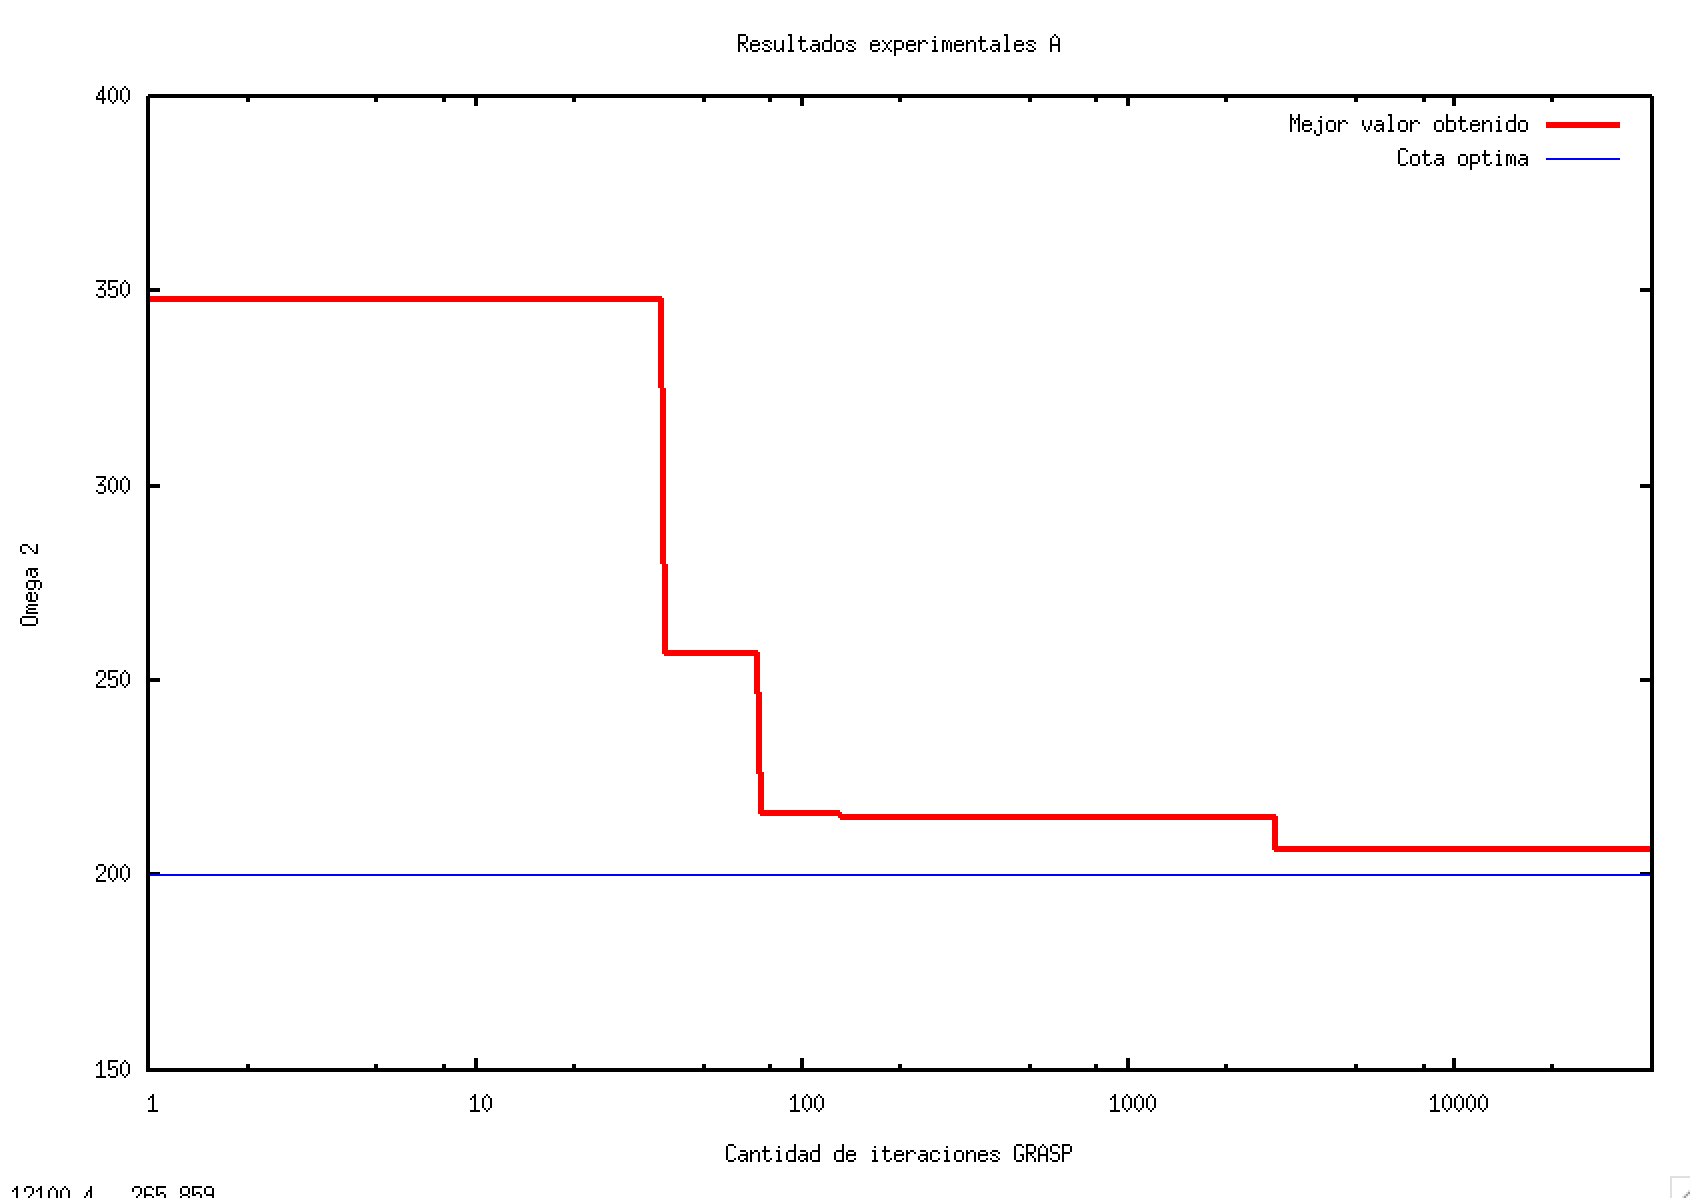
\includegraphics[angle=0, scale=.5]{imagenes/iteraciones-GRASP-A.png}
\label{Resultados experimentales A}
\end{center}
\end{figure}

\begin{figure}[H]
\begin{center}
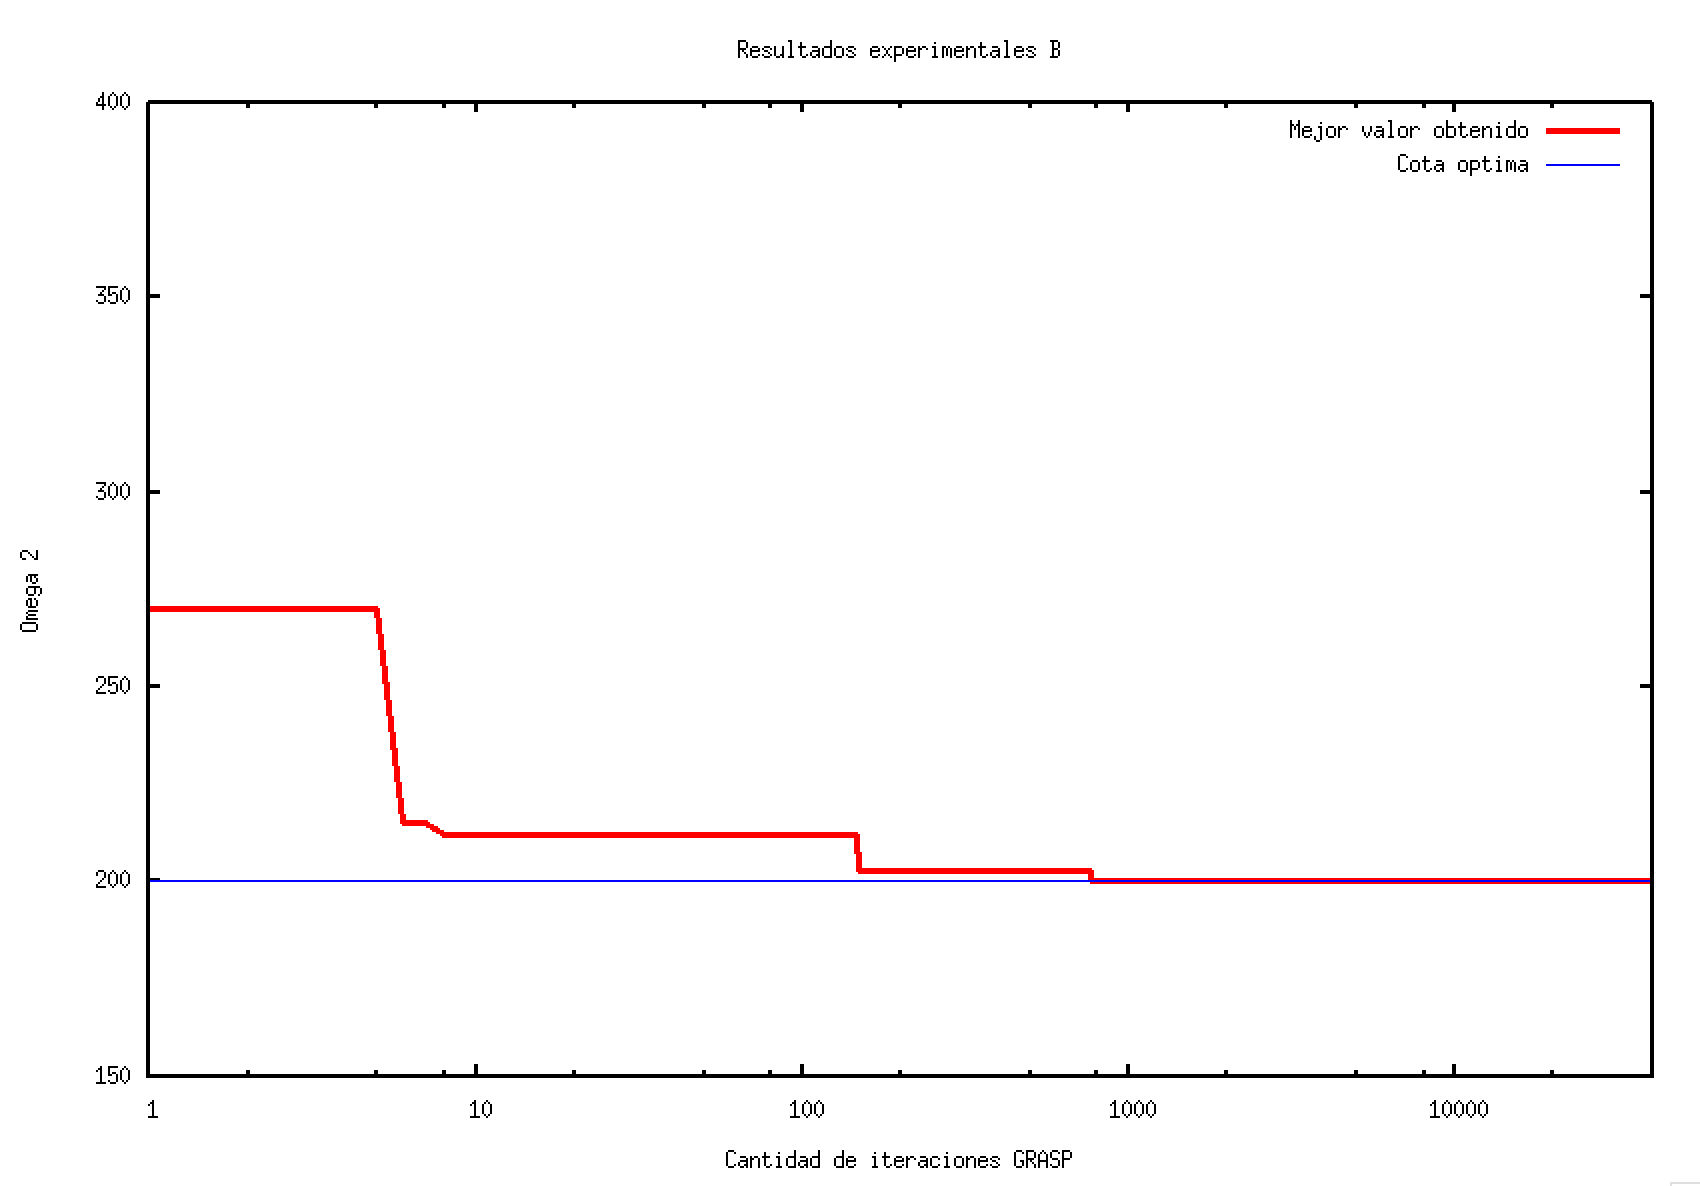
\includegraphics[angle=0, scale=.5]{imagenes/iteraciones-GRASP-B.png}
\label{Resultados experimentales A}
\end{center}
\end{figure}

\begin{figure}[H]
\begin{center}
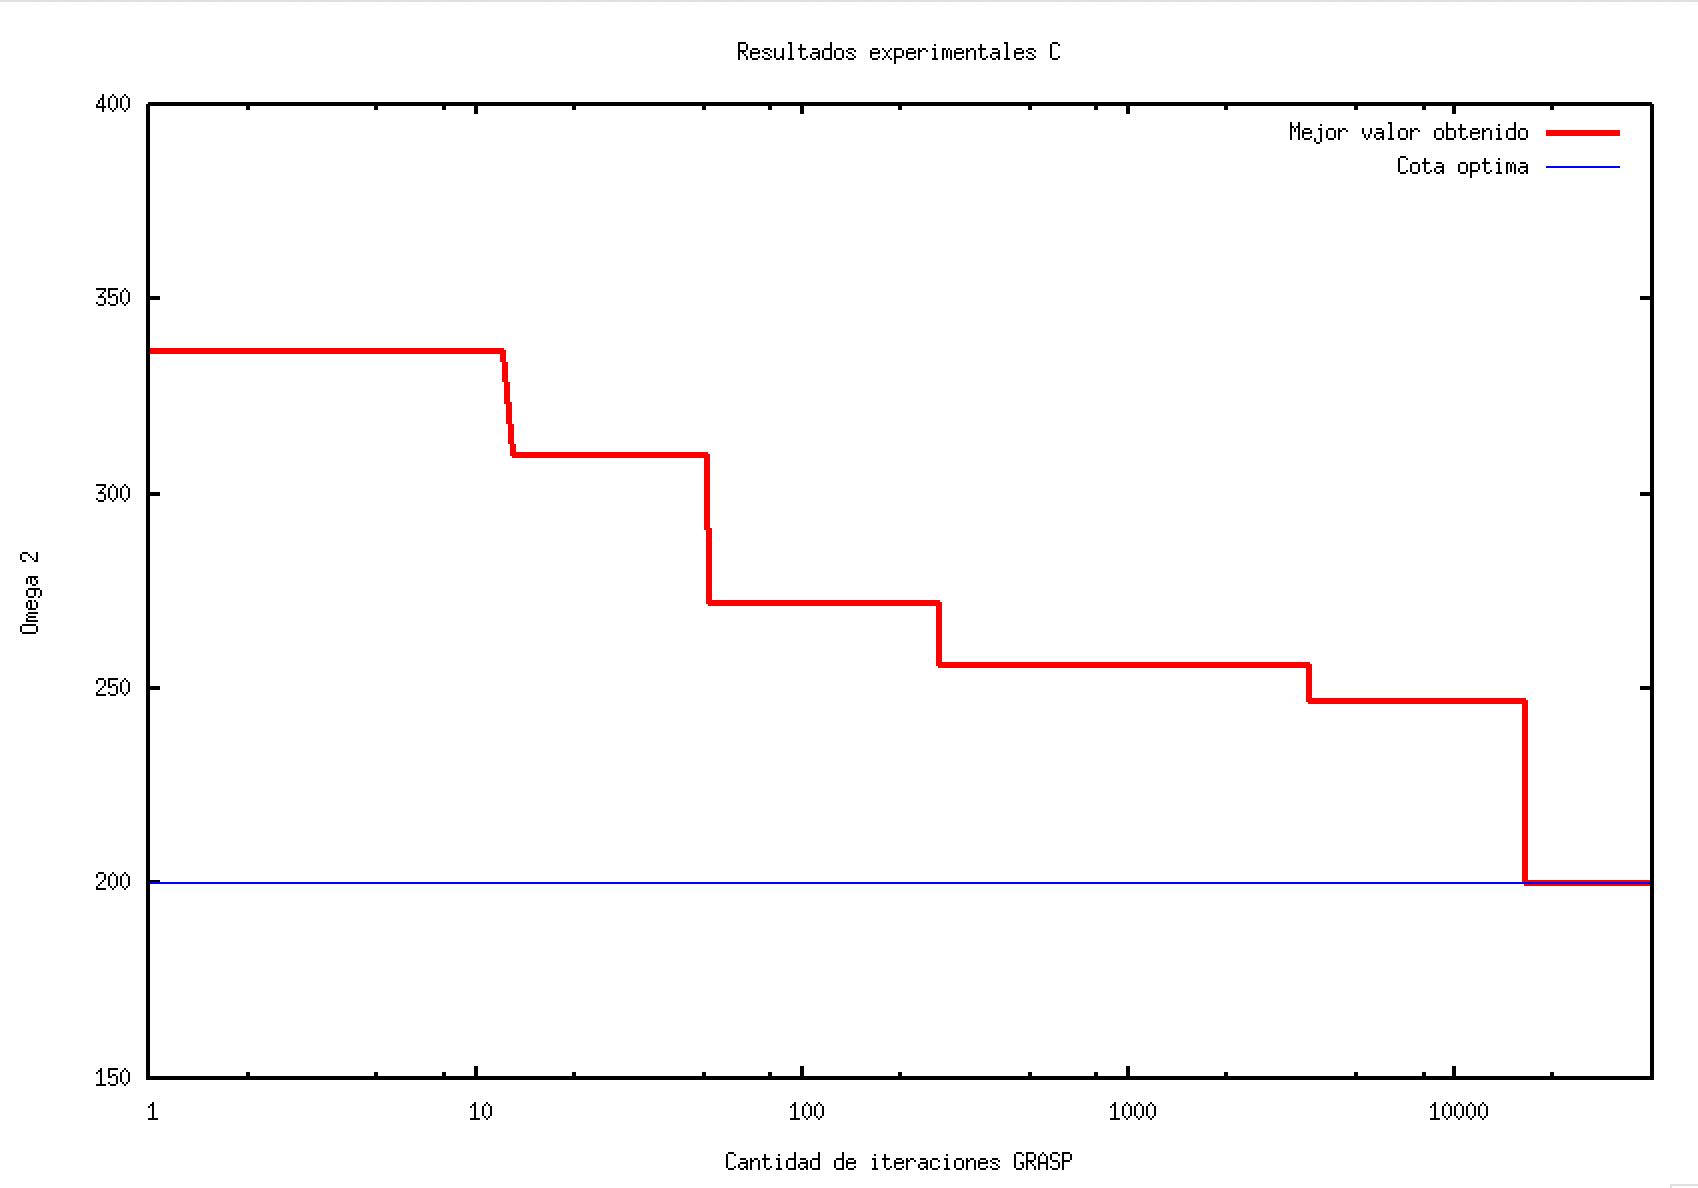
\includegraphics[angle=0, scale=.5]{imagenes/iteraciones-GRASP-C.png}
\label{Resultados experimentales C}
\end{center}
\end{figure}

Las experimentaciones A, B y C se realizaron corriendo GRASP usando grafos de entrada de 200 nodos y 400, 4000 y 10000 ejes respectivamente. Cada una de las experimentaciones ejecuta 40000 iteraciones\footnote{Se consideró que $n^2$ era una cantidad de iteraciones suficientemente grande como para realizar las pruebas. En caso de resultar insuficientes se realizaría una nueva prueba con una cantidad mayor.} en total, realizando en cada una un muestreo del valor de la mejor solución obtenida hasta el momento.

Cada figura muestra como evoluciona el valor de $\omega_2$ a medida que aumentan las iteraciones. Además, fue graficado el camino óptimo, cuya deducción es posible gracias a las características de los grafos utilizados, en donde para el mismo el valor de $\omega_2$ es igual a la cantidad de nodos del grafo, menos uno, es decir 199. De esta forma, pudimos comparar cuán buenos fueron los valores obtenidos.

Luego de tomar las muestras, dada la naturaleza de los datos obtenidos, decidimos utilizar escala logarítmica en el eje X para facilitar la visualización de los resultados, ya que como característica general notamos que se presenta una veloz \textit{mejoría} en las soluciones durante las primeras iteraciones. Esta característica se encuentra fuertemente acentuada en los \textbf{experimentos A y B}, en los que se puede observar que durante las \textbf{primeras 1000 iteraciones}, es decir el primer $2,5\%$ del muestreo total, la \textbf{distancia a la solución óptima} realiza una disminución crítica, de $150$ a $10$ en el caso del \textbf{experimento A}, y de $70$ a $0$ en el caso del \textbf{experimento B}. El \textbf{experimento C}, también demuestra una notable mejoría en la distancia a la solución óptima, de $150$ a $50$, en el transcurso de las primeras 1000 iteraciones; la misma es, sin embargo, mucho más escalonada. La vertiginosa velocidad de acercamiento al valor óptimo (en comparación con la cantidad de iteraciones realizadas) justificó la utilización de esta escala. 

Nuestro objetivo al momento de considerar los valores óptimos para los criterios de parada se basó en encontrar una forma de elegirlos de manera tal que los mismos se adecúen correctamente a grafos de variada densidad. 

Creando grafos con una cantidad fija y representativa de nodos, y variando la densidad de aristas de los mismos, encontramos que para el caso de grafos de 200 vértices, el algoritmo puede iterar aproximadamente 10000 iteraciones \textbf{sin encontrar mejoras}. Este valor lo obtuvimos del anteúltimo salto de la \textbf{experimentación C}, y se corresponde con $n^2 / 4$.

La \textbf{máxima cantidad de iteraciones necesarias} para encontrar un \textbf{valor considerablemente cercano al óptimo} fue observada también en la \textbf{experimentación C}, siendo esta de alrededor de 20000 iteraciones, o $n^2 / 2$.

Para elegir un valor para la \textbf{cantidad máxima de iteraciones que pueden transcurrir sin haber encontrado una solución inicial factible}, tomamos el mismo valor que para la cantidad máxima de iteraciones sin haber encontrado mejoras, es sea $n^2 / 4$. Esto se fundamenta en que si no se encontró una solución inicial factible, tampoco se mejoró la última solución encontrada y por ende este criterio nos sirve para acotar el valor.

Además de encontrar valores que consideramos útiles y adecuados para los ya mencionados criterios, encontramos interesante la influencia de la densidad de los grafos en el comportamiento del algoritmo. Dada una entrada de baja densidad de aristas, es más difícil que el mismo encuentre una buena solución inicial, y más aún \textbf{mejorar una solución relativamente cercana al óptimo} (en el muestreo concreto se puede observar que transcurren unas 39000 iteraciones, las últimas, en donde sólo se sucede una pequeña mejora de la solución). Dedujimos que esto sucede porque en la el grafo A hay pocos caminos (dada la baja densidad) y por consiguiente hay menos chances de encontrar los \textbf{mejores caminos}. Creemos que por esto sucede que no se logra llegar al óptimo aún luego de correr 40000 iteraciones, y por tal motivo creemos que llegado este punto es inútil seguir intentando encontrar un camino mejor.

El experimento que muestra el mejor comportamiento del algoritmo es el B, usando densidad media. Logra encontrar el camino óptimo mucho antes de llegar a nuestra cota para la cantidad de iteraciones: tarda alrededor de 1000 iteraciones (muy por debajo de las 20000($n^2 / 2$) iteraciones que utilizaremos finalmente como cota máxima). Además, logra encontrar un camino inicial bastante mejor que las otras dos opciones($\omega_2$ = 250 frente a $\omega_2$=300+ de A y C, es decir un $25\%$ mejor dado el óptimo de 200). 

Por último, creemos que la experimentación C muestra un caso representativo de la gran filosofía GRASP, ya que se que mejora la solución escalonadamente hasta dar con la óptima, luego de varias mejoras parciales.


\subsubsection{Búsqueda local}

La búsqueda local que realizamos es la misma que en el apartado anterior.

\subsubsection{Pseudocódigo}

El algoritmo está implementado en la función \texttt{main}:

\begin{algorithm}[H]
\caption{$main$(int tipo\_solucionInicial, Graph g, Nodo n1, Nodo n2)}
\begin{algorithmic}[1]
  \State crearMatrizCaminosMinimos(g)
  
  \State int $n = |nodes(g)|$
  \State int iteracionesSinMejorarCount = 0
  \State int iteracionesSinMejorarMax = n
  \State int iteracionesMax = $n \times log(n)$
  \State int iteracionesSinInitialPathCount = 0
  \State int iteracionesSinInitialPathMax = n
  \State mejorSolucion = NULL
  \For{i=0; i$<$iteracionesMax; i++}
  	\State Solution solucion = obtenerSolucionInicial(tipo\_solucionInicial, g, n1, n2)	
	\If{$\omega_1$(solucion) $>$ K}
    		\State iteracionesSinInitialPathCount++
		\If{iteracionesSinInitialPathCount $\geq$ iteracionesSinInitialPathMax}
			break
		\EndIf
        \EndIf

  
	\If{$\omega_1$(solucion) $\leq$ K}    
	    \While{True}    	        
	    	\State Solution nuevaSolucion = dameMejorVecino(solucion)
		\If{nuevaSolucion == NULL} 
			\State break	
		\EndIf    
		\State solucion = nuevaSolucion	
	    \EndWhile
	  
	  \If{mejorSolucion == NULL}
	  	\State mejorSolucion = solucion
	  \ElsIf{$\omega_2$(solucion) $<$ $\omega_2$(mejorSolucion)}
	  	\State mejorSolucion = solucion
	  \Else
	  	\State iteracionSinMejorarCount++
	  \EndIf
	\EndIf
	
	\If{iteracionesSinMejorarCount $>$ iteracionesSinMejorarMax}
                \State break
        \EndIf
	  
    \EndFor
\end{algorithmic}
\end{algorithm}

\begin{algorithm}[H]
\caption{$obtenerSolucionInicial$(int tipo, Graph g, Nodo n1, Nodo n2)}
\begin{algorithmic}[1]
  \If{tipo == Greedy\_C}
	\State return resolverConDijkstraAleatorio(g, n1, n2, ObjectiveFunctionC)
  \EndIf
  \State return resolverConDijkstraAleatorio(g, n1, n2, ObjectiveFunctionA)
\end{algorithmic}
\end{algorithm}

Las demás funciones tienen el mismo pseudocódigo que en Búsqueda local.

\subsubsection{Complejidad}

El algoritmo se ejecuta en un ciclo hasta cumplir con alguno de los criterios de terminación. Dado que el criterio de mayor valor es la cantidad de iteraciones totales($iteracionesMax$), tomamos ese valor como cota para calcular la complejidad.
Cada iteración del ciclo es casi idéntica a la ejecución de búsqueda local. La única diferencia es cómo se obtiene la solución inicial. Para encontrar la solución inicial se usa resolverConDijkstraAleatorio. Esta función, en vez de tomar el nodo no visitado con $\omega_2$ mínimo, toma uno entre los $beta$ menores. Pero resulta que la complejidad no se altera con este cambio, ya que Dijkstra itera sobre todos los nodos de cualquier manera y lo único que cambia es el orden en que se toma el nodo no visitado. 

Vale hacer una aclaración que es que como se usa una cola con prioridad para los nodos no visitados en Dijkstra, para sacar uno entre los $beta$ menores, se remueven los primeros $beta$ nodos de la cola y luego se agregan todos menos uno que es con el que nos quedamos. Como remover y agregar de la cola con prioridad toma $O(log(n))$, entonces para remover y agregar los $beta$ nodos se toma $O((beta + beta-1) \times log(n)) = O(\beta*log(n))$. Nosotros tomamos $\beta$ constante igual a 10.

Por lo tanto la complejidad de resolverConDijkstraAleatorio no resulta diferente resolverConDijkstra, usada en busqueda local y por ende la complejidad de cada iteración resulta igual a la complejidad de una ejecución de búsqueda local, o sea tiene complejidad $O(n^5)$.

Luego la complejidad total es $O(n^5  \times  iteracionesMax)$ = $O(n^5  \times  n \times log(n))$ = $O(n^6  \times  log(n))$.

\subsubsection{Experimentación}

A continuación presentamos los resultados de la experimentación del tiempo de ejecución de la metaheurística GRASP. Se utilizaron instancias del tipo \textit{mágico}, con una densidad media.

\begin{figure}[H]
\begin{center}
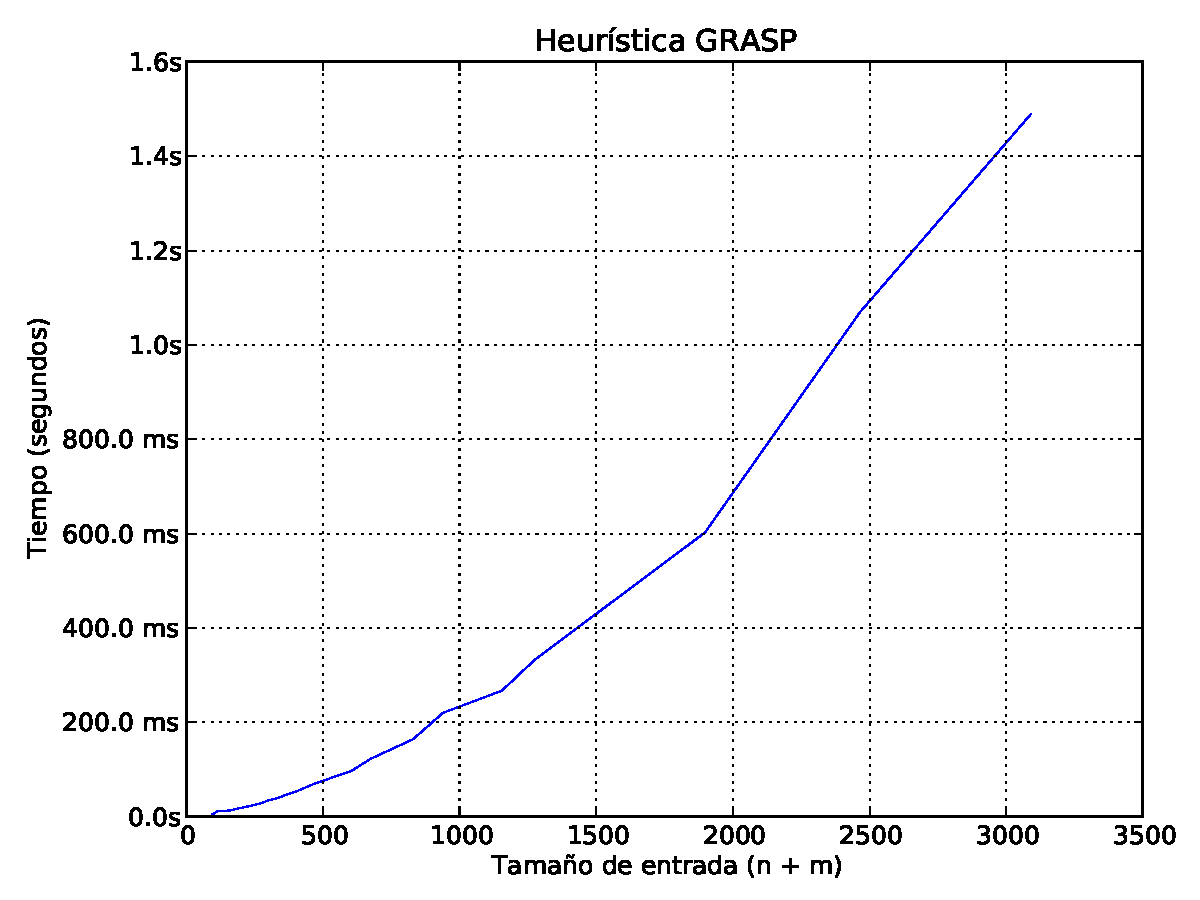
\includegraphics[angle=0, scale=.75]{imagenes/grasp_2014-06-27_19-18-59.pdf}
\label{grafico local}
\end{center}
\end{figure}

La curva que describe el tiempo de ejecución no evidencia un polinomio de grado 6, sin embargo, es evidente que tiene mucha más concavidad que la gráfica de la búsqueda
local. Ésto proviene  del hecho de repetir una cantidad que puede llegar a ser $n \times log(n)$ veces la búsqueda local.

Se prosigue la experimentación con la calidad de la solución.

\begin{figure}[H]
\begin{center}
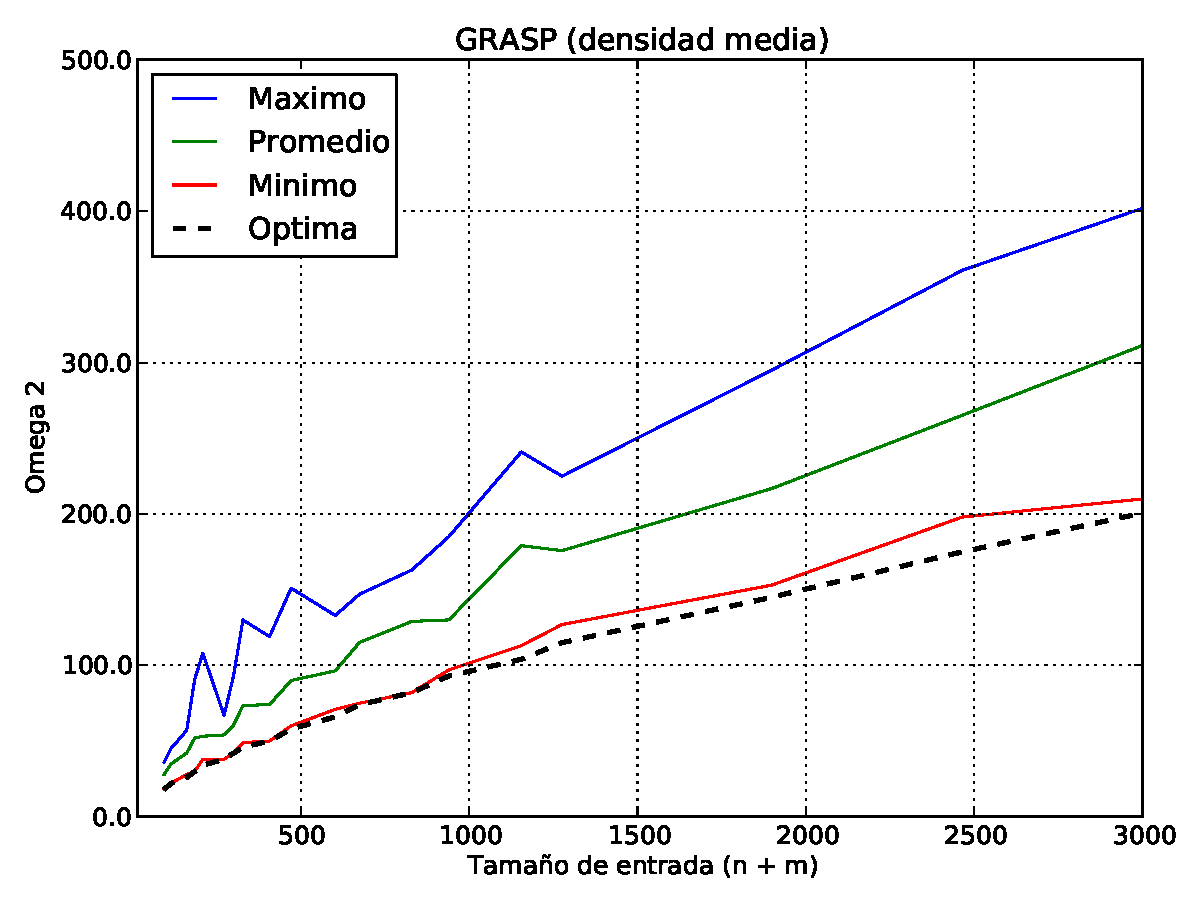
\includegraphics[angle=0, scale=.70]{imagenes/calidad_grasp_2014-06-27_08-58-53.pdf}
\label{grafico local}
\end{center}
\end{figure}

\begin{figure}[H]
\begin{center}
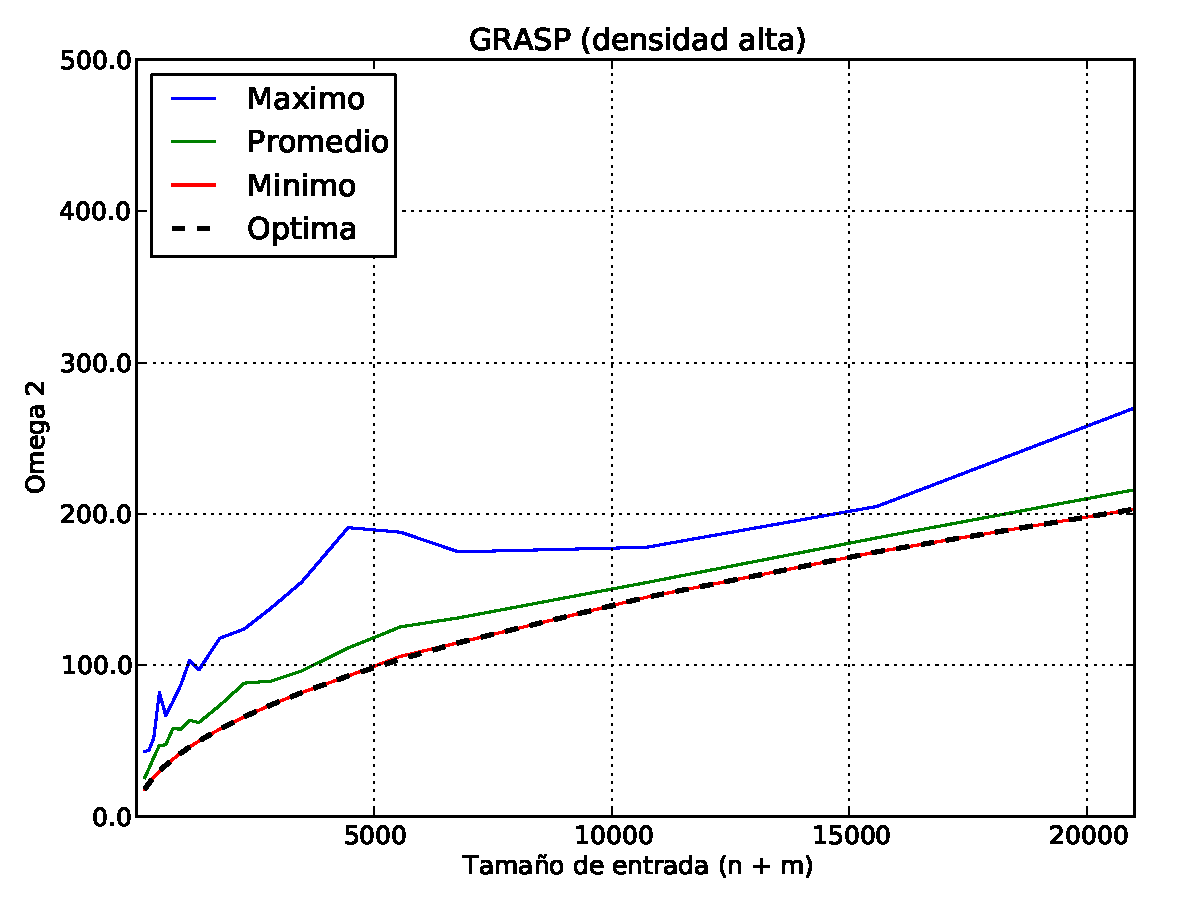
\includegraphics[angle=0, scale=.70]{imagenes/calidad_grasp_2014-06-27_08-54-46.pdf}
\label{grafico local}
\end{center}
\end{figure}

\newpage
La performance de GRASP nos llamó mucho la atención. Al igual que la búsqueda local, el resultado mínimo de nuestro algoritmo está muy cerca del
óptimo. Pero esta vez hemos logrado reducir la amplitud entre nuestros resultados y de esta forma acercar todo el cuerpo de nuestras soluciones
a la solución óptima.
Los buenos resultados obtenidos se deben a la naturaleza de GRASP, que consiste en iterativamente correr una búsqueda local sobre múltiples
soluciones iniciales generadas con un componente aleatorio. El repetir el experimento disminuye la varianza entre las diferentes corridas de GRASP y incrementa la posibilidad de una mejor solución
final.

  \newpage

%-- Apéndices --
\section{Apéndices}\label{sec:apendices}
  
  \subsection{Código Fuente (resumen)}\label{subsec:codigo-fuente}
  
\subsubsection{Backtracking}

\definecolor{gris}{rgb}{0.3,0.3,0.3}
\definecolor{rojito}{rgb}{1,0,0}
\lstset{language=C++,tabsize=2,basicstyle=\footnotesize,commentstyle=\color{gris},stringstyle=\color{rojito}}

\begin{lstlisting}[caption=backtracking.cpp]
Timer timer( cerr );

int main() {
    int N;
    while (cin >> N && N) {
        BacktrackingHeuristic b;
        b.parseInput(N);
        timer.setInitialTime( "todo_el_codigo" );
        
        if (b.U != b.V) {
            b.initialize();
            vector<Node> adjacent = b.G->getAdjacent(b.U); // se devuelve por referencia
            for (int i = 0; i < adjacent.size(); i++) {
                Node n = adjacent[i];
                Edge *f = b.G->getEdge(b.U, n);
                b.backtrack(f);
            }
        }
        
        timer.setFinalTime( "todo_el_codigo" );
        timer.saveAllTimes();
        b.printSolution();
    }
    return 0;
}
\end{lstlisting}
\begin{lstlisting}[caption=BacktrackingHeuristic::parseInput()]
void BacktrackingHeuristic::parseInput(int N) {
    this->N = N;
    cin >> this->M >> this->U >> this->V >> this->K;
    this->G = new Graph(N);
    this->visited = vector<bool>(N, false);
    int v1, v2;
    double w1, w2;
    for(int i = 0; i < M; i++) {
        cin >> v1 >> v2 >> w1 >> w2;
        this->G->addEdge(v1, v2, w1, w2);
    }
}
\end{lstlisting}
\begin{lstlisting}[caption=BacktrackingHeuristic::initialize()]
void BacktrackingHeuristic::initialize() {
    this->currentBranch.path.push_back(this->U);
    this->bestSolutionFound.totalOmega2 = INFINITE;
    
    DijkstraSolution byOmega1(N, V);
    DijkstraSolution byOmega2(N, V);
    Dijkstra<ObjectiveFunctionA> dijsktra1; 
    Dijkstra<ObjectiveFunctionB> dijsktra2; 
    dijsktra1.findPath(this->G, &byOmega1);
    dijsktra2.findPath(this->G, &byOmega2);
    this->distancesOmega1 = byOmega1.distances;
    this->distancesOmega2 = byOmega2.distances;
}
\end{lstlisting}
\begin{lstlisting}[caption=BacktrackingHeuristic::backtrack()]
void BacktrackingHeuristic::backtrack(Edge *e) {
    Node toNode = e->toNode;
    this->currentBranch.path.push_back(toNode);
    this->currentBranch.totalOmega1 += e->omega1;
    this->currentBranch.totalOmega2 += e->omega2;
    this->visited[toNode] = true;
    
    bool podar = ((this->currentBranch.totalOmega1 + this->distancesOmega1[toNode]) > this->K) ||
        ((this->currentBranch.totalOmega2 + this->distancesOmega2[toNode]) >= this->bestSolutionFound.totalOmega2);

    if (!podar) {
        if (toNode == this->V) {
            this->bestSolutionFound = currentBranch;
        } else {
            vector<Node> adjacent = G->getAdjacent(toNode); // se devuelve por referencia
            for (int i = 0; i < adjacent.size(); i++) {
                Node n = adjacent[i];
                if (!visited[n]) {
                    Edge *f = this->G->getEdge(toNode, n);
                    backtrack(f);
                }
            }
        }
    }

    this->currentBranch.path.pop_back();
    this->currentBranch.totalOmega1 -= e->omega1;
    this->currentBranch.totalOmega2 -= e->omega2;
    this->visited[toNode] = false;
}
\end{lstlisting}
\begin{lstlisting}[caption=BacktrackingHeuristic::printSolution()]
void BacktrackingHeuristic::printSolution() {
    Solution *s = &(this->bestSolutionFound);
    if (s->totalOmega2 == INFINITE) {
        cout << "no" << endl;
        return;
    }

    cout << s->totalOmega1 << " " << s->totalOmega2 << " " << (s->path.size()+1);
    for (int i = 0; i < s->path.size(); i++)
        cout << " " << s->path[i];
    cout << endl;
    return;
}
\end{lstlisting}
\subsubsection{Greedy}

\begin{lstlisting}[caption=greedy\_heuristic\_All.cpp]
#include <iostream>
#include "../common/Timer.h"
#include "GreedyHeuristicAll.h"

using namespace std;

int main(int argc, char* argv[])
{
  Timer timer(cerr);
  GreedyHeuristicAll greedy(&timer);
  greedy.run(); 
    
    return 0;
}
\end{lstlisting}
\begin{lstlisting}[caption=GreedyHeuristicAll.cpp]
#include "GreedyHeuristicAll.h"
#include "../common/Dijkstra.h"
#include "../common/ObjectiveFunctions.h"

GreedyHeuristicAll::GreedyHeuristicAll()
{
  solution = new Solution();
}

GreedyHeuristicAll::GreedyHeuristicAll(Timer* t)
{
  solution = new Solution();
  timer = t;
}
\end{lstlisting}
\begin{lstlisting}[caption=createSolutionA()]
Solution* createSolutionA(ProblemInstance* instance) 
{    
    // creo el dijkstra
    Dijkstra<ObjectiveFunctionA> dijsktra;
    // creo la solucion
    DijkstraSolution dijkstraSolution( instance->graph->nodeCount, instance->u);
    // cargo en la solucion, todos los paths del dijkstra desde el nodo inicial
    dijsktra.findPath( instance->graph, &dijkstraSolution );
    // obtengo el path que me interesa
    Solution* solution = new Solution();    
    dijkstraSolution.getPath( instance->v, instance->graph, solution->path, solution->totalOmega1, solution->totalOmega2 );
    return solution;
}
\end{lstlisting}
\begin{lstlisting}[caption=createSolutionB()]
Solution* createSolutionB(ProblemInstance* instance) 
{
    // creo el dijkstra    
    Dijkstra<ObjectiveFunctionB> dijsktra;
    // creo la solucion
    DijkstraSolution dijkstraSolution( instance->graph->nodeCount, instance->u);
    // cargo en la solucion, todos los paths del dijkstra desde el nodo inicial
    dijsktra.findPath( instance->graph, &dijkstraSolution );
    // obtengo el path que me interesa
    Solution* solution = new Solution();    
    dijkstraSolution.getPath( instance->v, instance->graph, solution->path, solution->totalOmega1, solution->totalOmega2 );
    return solution;
}
\end{lstlisting}
\begin{lstlisting}[caption=createSolutionC()]
Solution* createSolutionC(ProblemInstance* instance) 
{
    // creo el dijkstra    
    Dijkstra<ObjectiveFunctionC> dijsktra;
    // creo la solucion
    DijkstraSolution dijkstraSolution( instance->graph->nodeCount, instance->u);
    // cargo en la solucion, todos los paths del dijkstra desde el nodo inicial
    dijsktra.findPath( instance->graph, &dijkstraSolution );
    // obtengo el path que me interesa
    Solution* solution = new Solution();    
    dijkstraSolution.getPath( instance->v, instance->graph, solution->path, solution->totalOmega1, solution->totalOmega2 );
    return solution;
}
\end{lstlisting}
\begin{lstlisting}[caption=getBestSolution()]
Solution* getBestSolution(ProblemInstance* instance) 
{
    Solution* solutionB = createSolutionB(instance);    
    if(solutionB->totalOmega1 <= instance->K) {
        return solutionB;
    }
    //cout << "K " << instance->K << endl;
    //cout << "solutionB omega1 " << solutionB->totalOmega1 << endl;
    // si la solucion no es factible probamos con otras funciones objetivo    
    Solution* solutionA = createSolutionA(instance);
    Solution* solutionC = createSolutionC(instance);
    if(solutionC->totalOmega1 <= instance->K) {
        if(solutionA->totalOmega2 < solutionC->totalOmega2) {            
            return solutionA;
        }         
        return solutionC;
    }    

    //cout << "solutionC omega1 " << solutionC->totalOmega1 << endl;

    if(solutionA->totalOmega1 <= instance->K) {
        return solutionA;
    }
    //cout << "solutionA omega2 " << solutionA->totalOmega2 << endl;
    return NULL;   
}
\end{lstlisting}
\begin{lstlisting}[caption=GreedyHeuristicAll::resolveInstance()]
void GreedyHeuristicAll::resolveInstance( ProblemInstance* instance ){
  solution = getBestSolution(instance);
}
\end{lstlisting}
\begin{lstlisting}[caption=GreedyHeuristicAll::run()]
void GreedyHeuristicAll::run()
{
  Parser parser;
  parser.parseInput();

  for ( int i = 0; i < parser.problemInstances.size(); i++ )
  {
    ProblemInstance* instance = parser.problemInstances[i];
    
    timer->setInitialTime("todo_el_codigo");
    resolveInstance( instance );       
    timer->setFinalTime("todo_el_codigo");
    timer->saveAllTimes();
    
    if(!solution) {
      cout << "no" << endl;
    } else{
      solution->print();
    }    
  }
}
\end{lstlisting}

\subsubsection{Local Search}

\begin{lstlisting}[caption=local\_search.cpp]
#include "../common/Graph.h"
#include "../common/Parser.h"
#include "../common/DijkstraSolution.h"
#include "../common/Dijkstra.h"
#include "../common/GreedyHeuristic.h"
#include "../common/Solution.h"
#include "../common/Parser.h"
#include "../common/Timer.h"
#include "NeighbourhoodSelectorA.h"
#include "InitialSolution.h"

Parser parser;
Timer timer( cerr );


int main( int argc, char const* argv[] )
{
  /*****************
    Initialization
  ******************/
  // instantiate the initial solution using the initial solution parameter
  InitialSolution* initialSolution = new InitialSolution();
  // instantiate the neighborhood selector using the neighborhood selector parameter
  NeighbourhoodSelector* selector = new NeighbourhoodSelectorA();
  // parse the input
  parser.parseInput();

  /*************************
    Iterate over instances
  *******************'*******/
  for(auto instance:parser.problemInstances)
  {
    /*************
      Resolution
    **************/
    selector->initialize(instance);

    // obtain the initial time
    timer.setInitialTime( "todo_el_codigo" );
    // obtain the initial solution

    int initialSolutionOmega2;

    Solution* solution = initialSolution->getInitialSolution( instance );
    //cout << "Initial solution: ";


    // El dijkstra de omega1 debe cumplir con el K, sino no tiene sentido correr la heuristica
    // si solution no es valida entonces, entonces es NULL
    if(solution != NULL) {
      initialSolutionOmega2 = solution->totalOmega2;

      // run the heuristic
      Solution* newSolution = NULL;
      bool huboMejora = false;
      do
      {
        newSolution = selector->getBestNeighbour( solution );
        // Si no logro mejorar la solucion, termino
        if(newSolution != NULL) {
          //cout << "Mejore omega2!" << endl;
          //cout << "new solution: ";
          //newSolution->print();
          delete solution;
          solution = newSolution;          
          huboMejora = true;  
        } else {                      
          huboMejora = false;
        }
      } while(huboMejora);
    } 

    // obtain the final time
    timer.setFinalTime( "todo_el_codigo" );

    /***************
      Output Print
    ****************/
    // print the solution
    //cout << "Final solution: ";
    if(solution) {
      solution->print();
      delete solution;
    }
    else
    {
      cout << 0 << endl;
    }
    //solution->printTP();

    // save all obtained times to output
    timer.saveAllTimes();
  }
  return 0;
}
\end{lstlisting}
\begin{lstlisting}[caption=createSolutionA()]
Solution* createSolutionA(ProblemInstance* instance) 
{    
    // creo el dijkstra
    Dijkstra<ObjectiveFunctionA> dijsktra;
    // creo la solucion
    DijkstraSolution dijkstraSolution( instance->graph->nodeCount, instance->u);
    // cargo en la solucion, todos los paths del dijkstra desde el nodo inicial
    dijsktra.findPath( instance->graph, &dijkstraSolution );
    // obtengo el path que me interesa
    Solution* solution = new Solution();    
    dijkstraSolution.getPath( instance->v, instance->graph, solution->path, solution->totalOmega1, solution->totalOmega2 );
    return solution;
}
\end{lstlisting}
\begin{lstlisting}[caption=createSolutionB()]
Solution* createSolutionB(ProblemInstance* instance) 
{
    // creo el dijkstra    
    Dijkstra<ObjectiveFunctionB> dijsktra;
    // creo la solucion
    DijkstraSolution dijkstraSolution( instance->graph->nodeCount, instance->u);
    // cargo en la solucion, todos los paths del dijkstra desde el nodo inicial
    dijsktra.findPath( instance->graph, &dijkstraSolution );
    // obtengo el path que me interesa
    Solution* solution = new Solution();    
    dijkstraSolution.getPath( instance->v, instance->graph, solution->path, solution->totalOmega1, solution->totalOmega2 );
    return solution;
}
\end{lstlisting}
\begin{lstlisting}[caption=createSolutionC()]
Solution* createSolutionC(ProblemInstance* instance) 
{
    // creo el dijkstra    
    Dijkstra<ObjectiveFunctionC> dijsktra;
    // creo la solucion
    DijkstraSolution dijkstraSolution( instance->graph->nodeCount, instance->u);
    // cargo en la solucion, todos los paths del dijkstra desde el nodo inicial
    dijsktra.findPath( instance->graph, &dijkstraSolution );
    // obtengo el path que me interesa
    Solution* solution = new Solution();    
    dijkstraSolution.getPath( instance->v, instance->graph, solution->path, solution->totalOmega1, solution->totalOmega2 );
    return solution;
}
\end{lstlisting}
\begin{lstlisting}[caption=InitialSolution::getInitialSolution()]
Solution* InitialSolution::getInitialSolution(ProblemInstance* instance)
{   
    Solution* solutionB = createSolutionB(instance);    
    if(solutionB->totalOmega1 <= instance->K) {
        return solutionB;
    }
    // si la solucion no es factible probamos con otras funciones objetivo    
    Solution* solutionA = createSolutionA(instance);
    Solution* solutionC = createSolutionC(instance);
    if(solutionC->totalOmega1 <= instance->K) {
        if(solutionA->totalOmega2 < solutionC->totalOmega2) {
            return solutionA;
        } 
        return solutionC;
    }
    if(solutionA->totalOmega1 <= instance->K) {
        return solutionA;
    }
    return NULL;    
}
\end{lstlisting}
\begin{lstlisting}[caption=NeighbourhoodSelectorA::removeCycles()]
Solution* NeighbourhoodSelectorA::removeCycles(Solution* solution) 
{
  int* nextNodes = new int[nodeCount];
  for(int i=0; i<nodeCount; i++) {
    nextNodes[i] = 0;
  }  
  for(unsigned int i=0; i<solution->path.size(); i++) {
    Edge* edge = solution->path[i];    
    nextNodes[edge->fromNode] = edge->toNode;        
  }        

  vector<int> newPath;
  int firstNode = solution->path[0]->fromNode;
  int lastNode = solution->path[solution->path.size()-1]->toNode;  
  int next = firstNode;
  newPath.push_back(firstNode);     
  int a = 0;
  while(nextNodes[next] != lastNode)
  {    
    next = nextNodes[next];        
    newPath.push_back(next);    
  }

  newPath.push_back(lastNode);
  //cout << lastNode << endl;
  
  Solution* newSolution = new Solution();
  for(int i=0; i<newPath.size()-1; i++){    
    Edge* edge = solution->getEdgeBetween(newPath[i], newPath[i+1]);    
    Edge* newEdge = new Edge(edge->fromNode, edge->toNode, edge->omega1, edge->omega2);
    newSolution->path.push_back(newEdge);
    newSolution->totalOmega1 += newEdge->omega1;
    newSolution->totalOmega2 += newEdge->omega2;
  }

  return newSolution;
}
\end{lstlisting}
\begin{lstlisting}[caption=createNewSolutionReplacingPath()]
Solution* createNewSolutionReplacingPath(const Solution* orig, const Solution* sub) {
  int node1 = sub->path[0]->fromNode;
  int node2 = sub->path[sub->path.size()-1]->toNode;
  Solution* res = new Solution();
  vector<Edge*> edgesToRemove;
  bool subPathStartsAtNode1 = false;
  int subPathStartsAtEdgeIndex = 0;
  // primero agrego todos los edges del path original hasta encontrar alguno de los nodos del subpath
  for(int i=0; i<orig->path.size(); i++) {
    Edge* edge = orig->path[i];
    if(edge->fromNode == node1 || edge->fromNode == node2) {
      subPathStartsAtNode1 = edge->fromNode == node1;
      subPathStartsAtEdgeIndex = i;
      break;
    } else {
      res->path.push_back(edge);
      res->totalOmega1 += edge->omega1;
      res->totalOmega2 += edge->omega2;
    }
  }

  // agrego todos los ejes del sub path
  for(int i=0; i<sub->path.size(); i++) {
    Edge* edge = sub->path[i];
    res->path.push_back(edge);
    res->totalOmega1 += edge->omega1;
    res->totalOmega2 += edge->omega2;
  }

  // busco el nodo desde donde continua el pedazo del path original
  // agrego todos los ejes del path original a partir de ahi
  int fromNode = subPathStartsAtNode1 ? node2 : node1;
  bool addEdges = false;
  for(int i=subPathStartsAtEdgeIndex+1; i<orig->path.size(); i++) {
    Edge* edge = orig->path[i];
    if(edge->fromNode == fromNode) {
      addEdges = true; // encontre el nodo, asi que comienzo a aniadir los nodos desde aca
    }
    if(addEdges) {
      res->path.push_back(edge);
      res->totalOmega1 += edge->omega1;
      res->totalOmega2 += edge->omega2;
    }
  }

  return res;
}
\end{lstlisting}
\begin{lstlisting}[caption=NeighbourhoodSelectorA::getBestNeighbour()]
Solution* NeighbourhoodSelectorA::getBestNeighbour(const Solution* origSolution)
{ 
  // Itero sobre la matriz de soluciones
  // Por cada par de nodos, tengo que buscar si existe un path en la matriz, 
  // tal que sustituyendolo pot path entre el par de nodos de la solucion original 
  // se obtenga una nueva solucion tal que se su totalOmega2 sea menor
  
  // Nota: Habiamos pensado en usar DeltaOmega2, pero si K es muy grande,
  // nos sobraria mucho K que podriamos haber usado para sustituir en cada paso
  // por un path con minimo omega2                
  
  // El path de una solution es un vector de ejes   
  // En cada iteracion que encuentro una solucion mejor, voy a cambiar algunos de los nodos, 
  // por lo que tengo que recalcular los nodos de la mejor solucion             
  int edgesCount = origSolution->path.size();
  int nodesCount = edgesCount+1;
  vector<int> nodes(nodesCount); 
  for(int i=0; i<edgesCount; i++) {
    Edge* edge = origSolution->path[i];
    nodes[i] = edge->fromNode;
  }
  nodes[nodesCount-1] = origSolution->path[edgesCount-1]->toNode; // ultimo nodo del path
  //cout << endl;
      
  Solution* bestSolution = NULL;  
  for(int i=0; i<nodes.size() - 1; i++) {    
    for(int j=i+1; j<nodes.size(); j++) {           
      Solution* subSolution = origSolution->createSubSolutionBetween(nodes[i], nodes[j]); // solution con sub path entre los nodos            
      Solution* solution_ij = getSolvedPathBetween(nodes[i], nodes[j]); // dijkstra por omega2 entre los nodos
      if(solution_ij == NULL) {
        continue;
      }      
      /*cout << "Between (" << nodes[i] << ", " << nodes[j] << "):" << endl;
      cout << "subSolution: ";
      subSolution->print();
      cout << "solution_ij: ";
      solution_ij->print();*/
      
      // Si el path creado con dijkstra usando omega2, tiene menos omega2 total, que el path actual entre
      // los nodos i y j, entonces chequeo si al crear una nueva solucion tendra menos omega2 que la mejor solucion.
      // En ese caso me guardo esta nueva solucion como la mejor hasta ahora.
      // Ademas chequeo que se cumpla con el K requerido.                          
      double bestSolutionOmega2 = bestSolution == NULL ? origSolution->totalOmega2 : bestSolution->totalOmega2;
      double newSolutionOmega2 = origSolution->totalOmega2 - subSolution->totalOmega2 + solution_ij->totalOmega2;
      double newSolutionOmega1 = origSolution->totalOmega1 - subSolution->totalOmega1 + solution_ij->totalOmega1;            
      if(newSolutionOmega2 < bestSolutionOmega2 && newSolutionOmega1 <= K) {                     
        if(bestSolution != NULL) {
          delete bestSolution;   
        }       
        /*cout << "origSolution ";
        origSolution->print();
        cout << "subSolution ";
        subSolution->print();
        cout << "solution_ij ";
        solution_ij->print();*/
        // creo la nueva mejor solucion        
        bestSolution = createNewSolutionReplacingPath(origSolution, solution_ij);           
        /*cout << "bestSolution ";
        bestSolution->print();*/
        Solution* bestSolutionWithoutCycles = removeCycles(bestSolution);                         
        delete bestSolution;
        bestSolution = bestSolutionWithoutCycles;        
        //cout << "hubo mejora!" << endl;
        //cout << "bestSolution: ";
        //bestSolution->print();
      }      
      delete subSolution;

      //cout << endl;      
    }
  }
    
  return bestSolution;  
}
\end{lstlisting}
\subsubsection{Grasp}


\begin{lstlisting}[caption=grasp.cpp]
#include "../common/Graph.h"
#include "../common/Parser.h"
#include "../common/DijkstraSolution.h"
#include "../common/Dijkstra.h"
#include "../common/DijkstraRandomized.h"
#include "../common/GreedyHeuristic.h"
#include "../common/Solution.h"
#include "../common/Parser.h"
#include "../common/Timer.h"
#include "NeighbourhoodSelectorA.h"
#include "InitialSolution.h"
#include <math.h>

Parser parser;
Timer timer( cerr );


int main( int argc, char const* argv[] ) 
{
    /* Semilla random */
    srand (time(NULL));

    /*****************
      Initialization
    ******************/
            
    // parse the input
    parser.parseInput();  

    // obtain the initial time
    timer.setInitialTime( "todo_el_codigo" );
    // obtain the initial solution

    /*************************
      Iterate over instances
    **************************/
    for(auto instance:parser.problemInstances)
    {        
        /*************
         Resolution
        **************/           
        NeighbourhoodSelector* selector = new NeighbourhoodSelectorA();
        selector->initialize(instance);                        

        // valores arbitrarios basados en n para criterio de terminaciones
        int n = instance->graph->nodeCount;
        int iteracionesSinMejorarCount = 0;
        int iteracionesSinMejorarMax = n*n;//n;
        int iteracionesMax = n*n; //n * log(n);
        int iteracionesSinInitialPathCount = 0;
        int iteracionesSinInitialPathMax = n*n;//n;
        
        Solution* bestSolution = NULL;            

        for(int i = 0; i<iteracionesMax; i++) {  
            if(bestSolution) {
                cout << i << "\t" << bestSolution->totalOmega2 << endl;
            } else {
                cout << "0" << endl;
            }
            //cout <<  iteracionesSinMejorarCount << "/" << iteracionesSinMejorarMax << ", " <<
            //    i << "/" << iteracionesMax << ", " << 
            //    iteracionesSinInitialPathCount << "/" << iteracionesSinInitialPathMax << endl;
            // instantiate the initial solution using the initial solution parameter
            InitialSolution* initialSolution = new InitialSolution();              
            Solution* solution = initialSolution->getInitialSolution( instance );                     
            //solution->print();                  
            if(solution->path.size() == 0) {
                // no encontre un path entre u y v
                iteracionesSinInitialPathCount++;
                delete solution;            
                if(iteracionesSinInitialPathCount < iteracionesSinInitialPathMax) {
                    continue; // sigo intentando buscar soluciones
                } else {
                    break; // me rindo, dejo de buscar soluciones
                }            
            }                        
            //cout << "Initial solution: ";
            //solution->print();

            // El dijkstra de omega1 debe cumplir con el K, sino no tiene sentido correr la heuristica            
            if(solution->totalOmega1 <= instance->K) {                               
                // run the heuristic
                Solution* newSolution = NULL;    
                bool huboMejora = false;
                do
                {                                        
                    newSolution = selector->getBestNeighbour( solution );                                                            
                    // Si no logro mejorar la solucion, termino      
                    if(newSolution != NULL) {                        
                        //cout << newSolution->totalOmega2 << endl; 
                        delete solution;
                        solution = newSolution;          
                        huboMejora = true;                          
                    } else {                      
                        huboMejora = false;
                    }        
                } while(huboMejora);

                if(bestSolution == NULL) {
                    bestSolution = solution;
                } else if(solution->totalOmega2 < bestSolution->totalOmega2) {
                    //cout << "mejore la solucion! " << solution->totalOmega2 << endl;
                    //return 0;
                    delete bestSolution;
                    bestSolution = solution;
                } else {
                    delete solution;
                    iteracionesSinMejorarCount++;      
                }            
            }       

            if(iteracionesSinMejorarCount > iteracionesSinMejorarMax) {      
                break;
            }
        }  

        if(bestSolution) {
            //cout << bestSolution->totalOmega2 << endl;
        }

        // obtain the final time
        timer.setFinalTime( "todo_el_codigo" );

        /***************
          Output Print
        ****************/
        // print the solution
        if(bestSolution != NULL) {
            //cout << "Final solution: ";
            bestSolution->print();
            delete bestSolution;
        } else {
            cout << "no" << endl;
        }    
        
        // save all obtained times to output
        timer.saveAllTimes();

        //delete selector;
    }    
    
    return 0;
}
\end{lstlisting}
\begin{lstlisting}[caption=InitialSolution::getInitialSolution()]
Solution* InitialSolution::getInitialSolution(ProblemInstance* instance)
{    
  // creo el dijkstra
    DijkstraRandomized<ObjectiveFunctionA> dijsktraRandom;
    // creo la solucion
    DijkstraSolution dijkstraSolution( instance->graph->nodeCount, instance->u);
    // cargo en la solucion, todos los paths del dijkstra desde el nodo inicial
    dijsktraRandom.findPath( instance->graph, &dijkstraSolution );
    // obtengo el path que me interesa
    Solution* solution = new Solution();    
    dijkstraSolution.getPath( instance->v, instance->graph, solution->path, solution->totalOmega1, solution->totalOmega2 );
    return solution;
}
\end{lstlisting}
  \clearpage
  
  %
  % - Para la reentrega -
  %
  %\subsection{Informe de Modificaciones}
  %\begin{itemize}
    \item Se revisaron en general todas las secciones de acuerdo a las correcciones.
    \item Se agregaron dos nuevas secciones: \textit{Pautas generales de medición} y \textit{Pautas para la generación de grafos}.
\end{itemize}

  %\clearpage
  
  %-- Bibliografia --
  %\subsection{Bibliografía}
  %\begin{thebibliography}{99}
% 
%   \bibitem{lib:brassard} G. Brassard, P. Bratley, \textit{Fundamental of Algorithmics}, Prentice Hall,  1996, Chapter 6.2, \enquote{General characteristics of greedy algoritmhs}, Chapter 9.6, \enquote{Backtracking}, 
%   \bibitem{lib:cormen} Cormen, Leiserson, Rivest \textit{Introduction to Algorithms}, 2001, Chapter 16 \enquote{Greedy Algorithms}.
%   \bibitem{stl:stl} \texttt{http://www.cplusplus.com/reference/stl/}
%   \bibitem{stl:set} \texttt{http://www.cplusplus.com/reference/set/set/}
%   \bibitem{stl:vector} \texttt{http://www.cplusplus.com/reference/vector/vector/}
%   \bibitem{stl:pqueue} \texttt{http://www.cplusplus.com/reference/queue/priority\_queue/}
%   \bibitem{wiki:greedy} \texttt{http://en.wikipedia.org/wiki/Greedy\_algorithm\#Specifics}
%   \bibitem{wiki:back} \texttt{http://en.wikipedia.org/wiki/Backtracking\#Usage\_considerations}

  %\end{thebibliography}

\end{TP3}
\end{document}
